\chapter{Common Definitions and Conventions}

\section{Coordinate Conventions}
The coordinate system of CMS is centered on the nominal interaction point. The
$x$-axis points towards the center of the LHC ring, the $y$-axis points certically
upwards and the $z$-axis points along the direction of the beamline, in the
anti-clockwise direction when the LHC is viewed from above. 
The azimuth angle, $\phi$, is the angle in the $x$-$y$ plane with respect to the
$x$-axis.  The polar angle, $\theta$, is measured from the $z$-axis.

The rapidity of a particle is defined as,
\begin{equation}
    y = \frac{1}{2} \ln \left(\frac{E+p_\text{L}}{E-p_\text{L}}\right),
\label{eq:rapidity}
\end{equation}
where $p_{L}$ is the longditudianl component (the component along the beam axis)
of the momentum of the particle. It represents the boost along the beam axis
required to go from the lab frame to the frame where the particle is produced
perpendicular to the beam axis.
The pseudorapidity is defined as 
\begin{equation}
    \eta = -\ln\left[\tan\left(\frac{\theta}{2}\right)\right], 
\label{eq:pseudorapidity}
\end{equation}
where $\theta$ is the polar angle.  In the massless approximation, this is equal
to the rapidity.

In CMS the initial longditudinal momentum in the event is not known. Many of the
kinematical quantaties are considered only in the transverse plane and denoted
with a `T' subscript, for example the transverse missing energy, \ETm, and the
transverse momentum, \pT.

\section{List of Acronyms}
\begin{center}
\begin{longtable}{ll}
ALICE\dotfill & A Large Ion Collider Experiment\\
APD\dotfill & Avalanche Photodiode\\
AS\dotfill & Anti-Selection\\
ATLAS\dotfill & A Toroidal LHC ApparatuS\\
CERN\dotfill & European Organization for Nuclear Research.\\
CMS\dotfill & Compact Muon Solenoid\\
CPU\dotfill & Central Processing Unit\\
CSC\dotfill & Cathode Strip Chamber\\
CTEQ\dotfill & The Coordinated Theoretical-Experimental Project on QCD\cite{lai2010vv}\\
DAQ\dotfill & Data Acquisition\\
DT\dotfill & Drift Tube\\
DY\dotfill & Drell-Yan\\
ECAL\dotfill & Electromagnetic Calorimeter\\
\ETm\dotfill & Missing Transverse Energy\\
EWSB\dotfill & Electroweak Symmetry Breaking\\
FSR\dotfill & Final State Radiation.\\
GSF\dotfill & Gaussian Sum Filter\\
HCAL\dotfill & Hadronic Calorimeter\\
HEP\dotfill & High Energy Physics\\
HERAPDF\dotfill & Hadron Elektron Ring Anlage PDF\cite{aaron2010combined} \\
HF\dotfill & Hadronic Calorimeter (Forward)\\
HLT\dotfill & High Level Trigger\\
KF\dotfill & Kalman Filter\\
L1\dotfill & Level 1 Trigger\\
LEP\dotfill & Large Electron-Positron Collider\\
LHAPDF\dotfill & Les Houches Accord PDF Interface\cite{whalley2005houches}\\
LHCb\dotfill & Large Hadron Collider Beauty.\\
LHC\dotfill & Large Hadron Collider\\
LINAC2\dotfill & Linear Accelerator 2\\
MC\dotfill & Monte Carlo\\
MCFM\dotfill & Monte Carlo for FeMtobarn processes\cite{campbellmcfm}\\
MET\dotfill & Missing Transverse Energy\\
MSTW\dotfill & Martin-Stirling-Thorne-Watt Parton Distribution Functions\cite{martin2009parton}\\
MVA\dotfill & Multivariate Analysis\\
NNPDF\dotfill & Neural Network Parton Distribution Functions\cite{Lionetti:2011pw}\\
NP\dotfill & New Physics\\
PDF\dotfill & Parton Distribution Function\\
PF\dotfill & Particle Flow\\
PFMET\dotfill & Particle Flow Missing Transverse Energy\\
PSB\dotfill & Proton Synchrotron Booster\\
PS\dotfill & Proton Synchrotron\\
PU\dotfill & Pile Up\\
PV\dotfill & Primary Vertex\\
QCD\dotfill & Quantum Chromo Dynamics\\
QED\dotfill & Quantum Electro Dynamics\\
RPC\dotfill & Resistive Plate Chamber\\
SM\dotfill & Standard Model\\
SPS\dotfill & Super Proton Synchrotron\\
SUSY\dotfill & Supersymmetry\\
TEC\dotfill & Tracker End Cap\\
TIB\dotfill & Tracker Inner Barrel\\
TID\dotfill & Tracker Inner Disk\\
TOB\dotfill & Tracker Outer Barrel.\\
TP\dotfill & Tag and Probe\\
VEV\dotfill & Vacuum Expectation Value\\
VPT\dotfill & Vacuum Phototriode\\
\end{longtable}
\end{center}



\chapter{Fits to the \ETm Distributions}
\section{\unit{36}{\invpb}}
\begin{figure}
\begin{center}
% bottom right top left
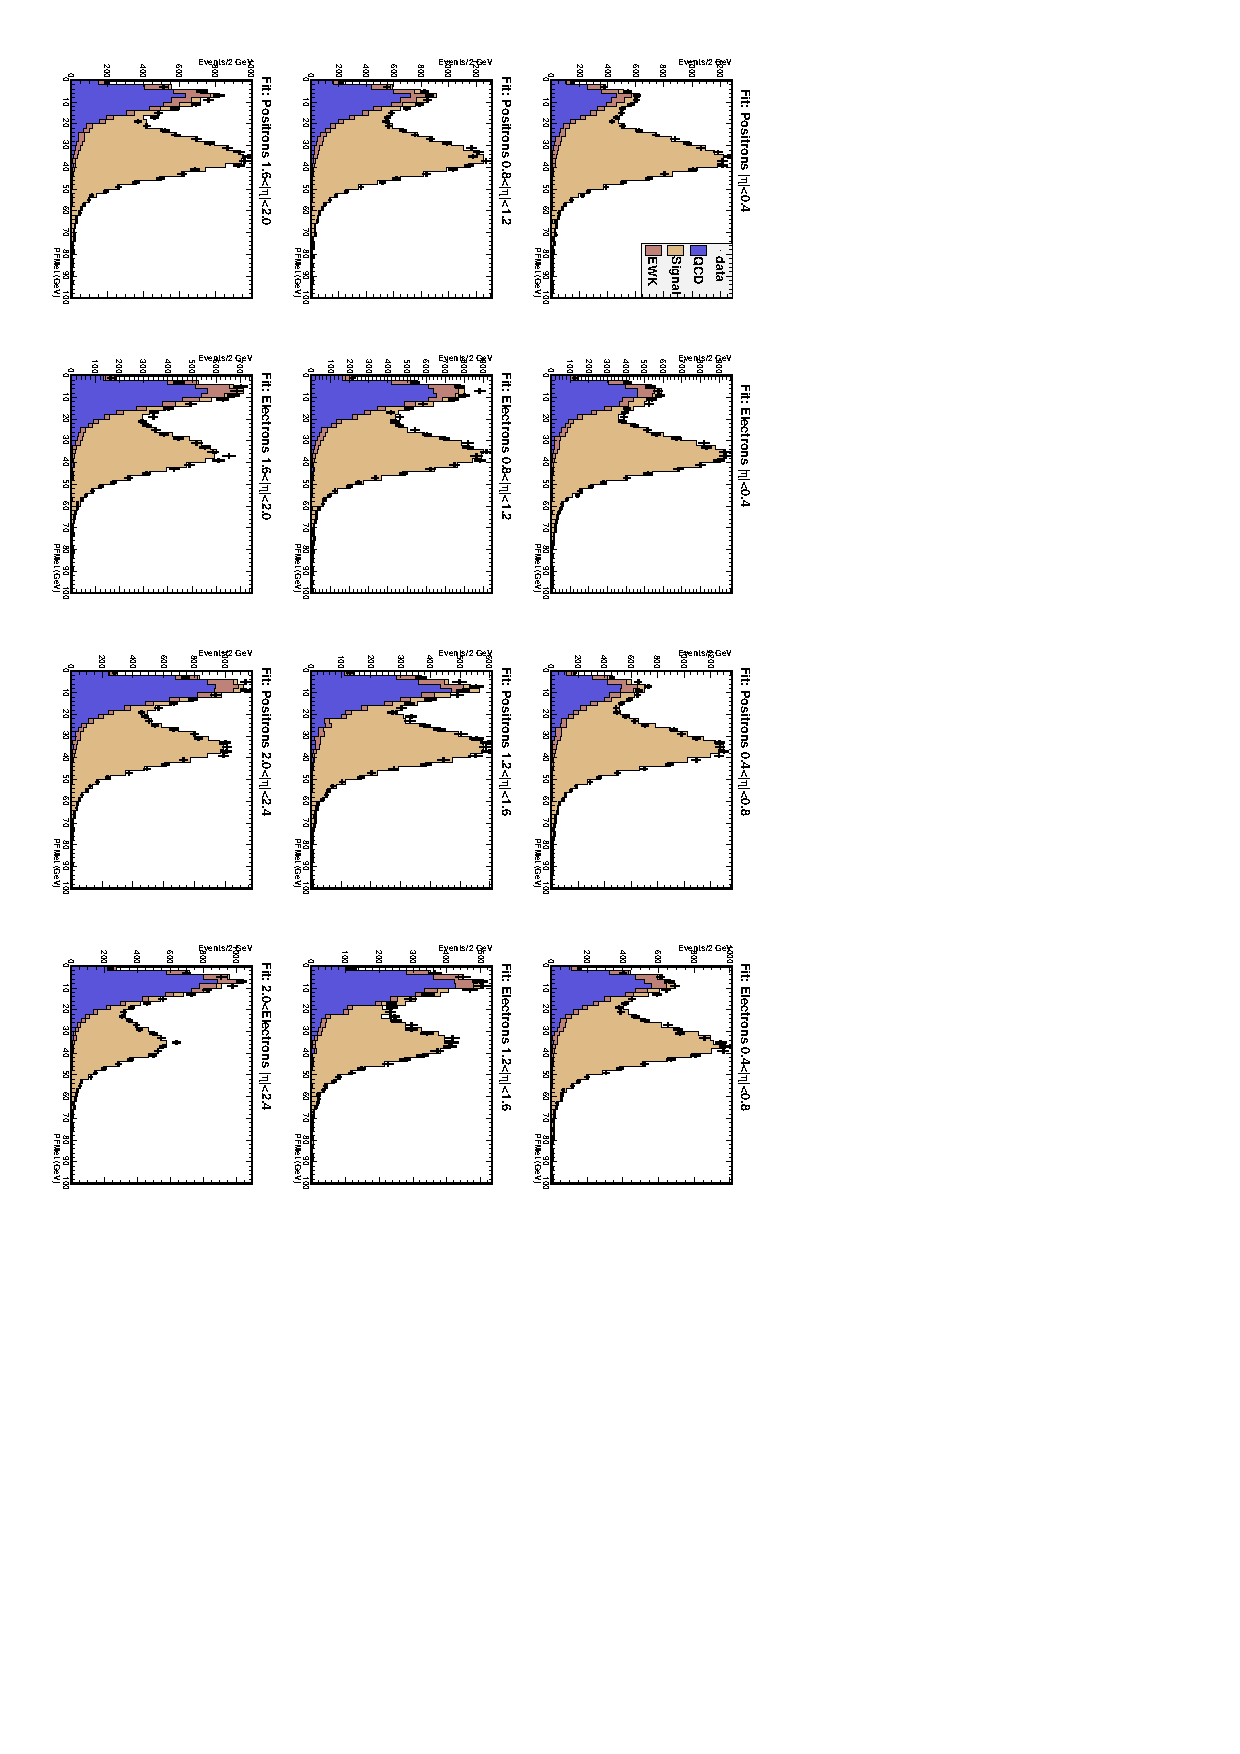
\includegraphics[trim = 80mm 100mm 0mm 0mm, clip, angle=90, width=0.95\textwidth]{Dec22_data}
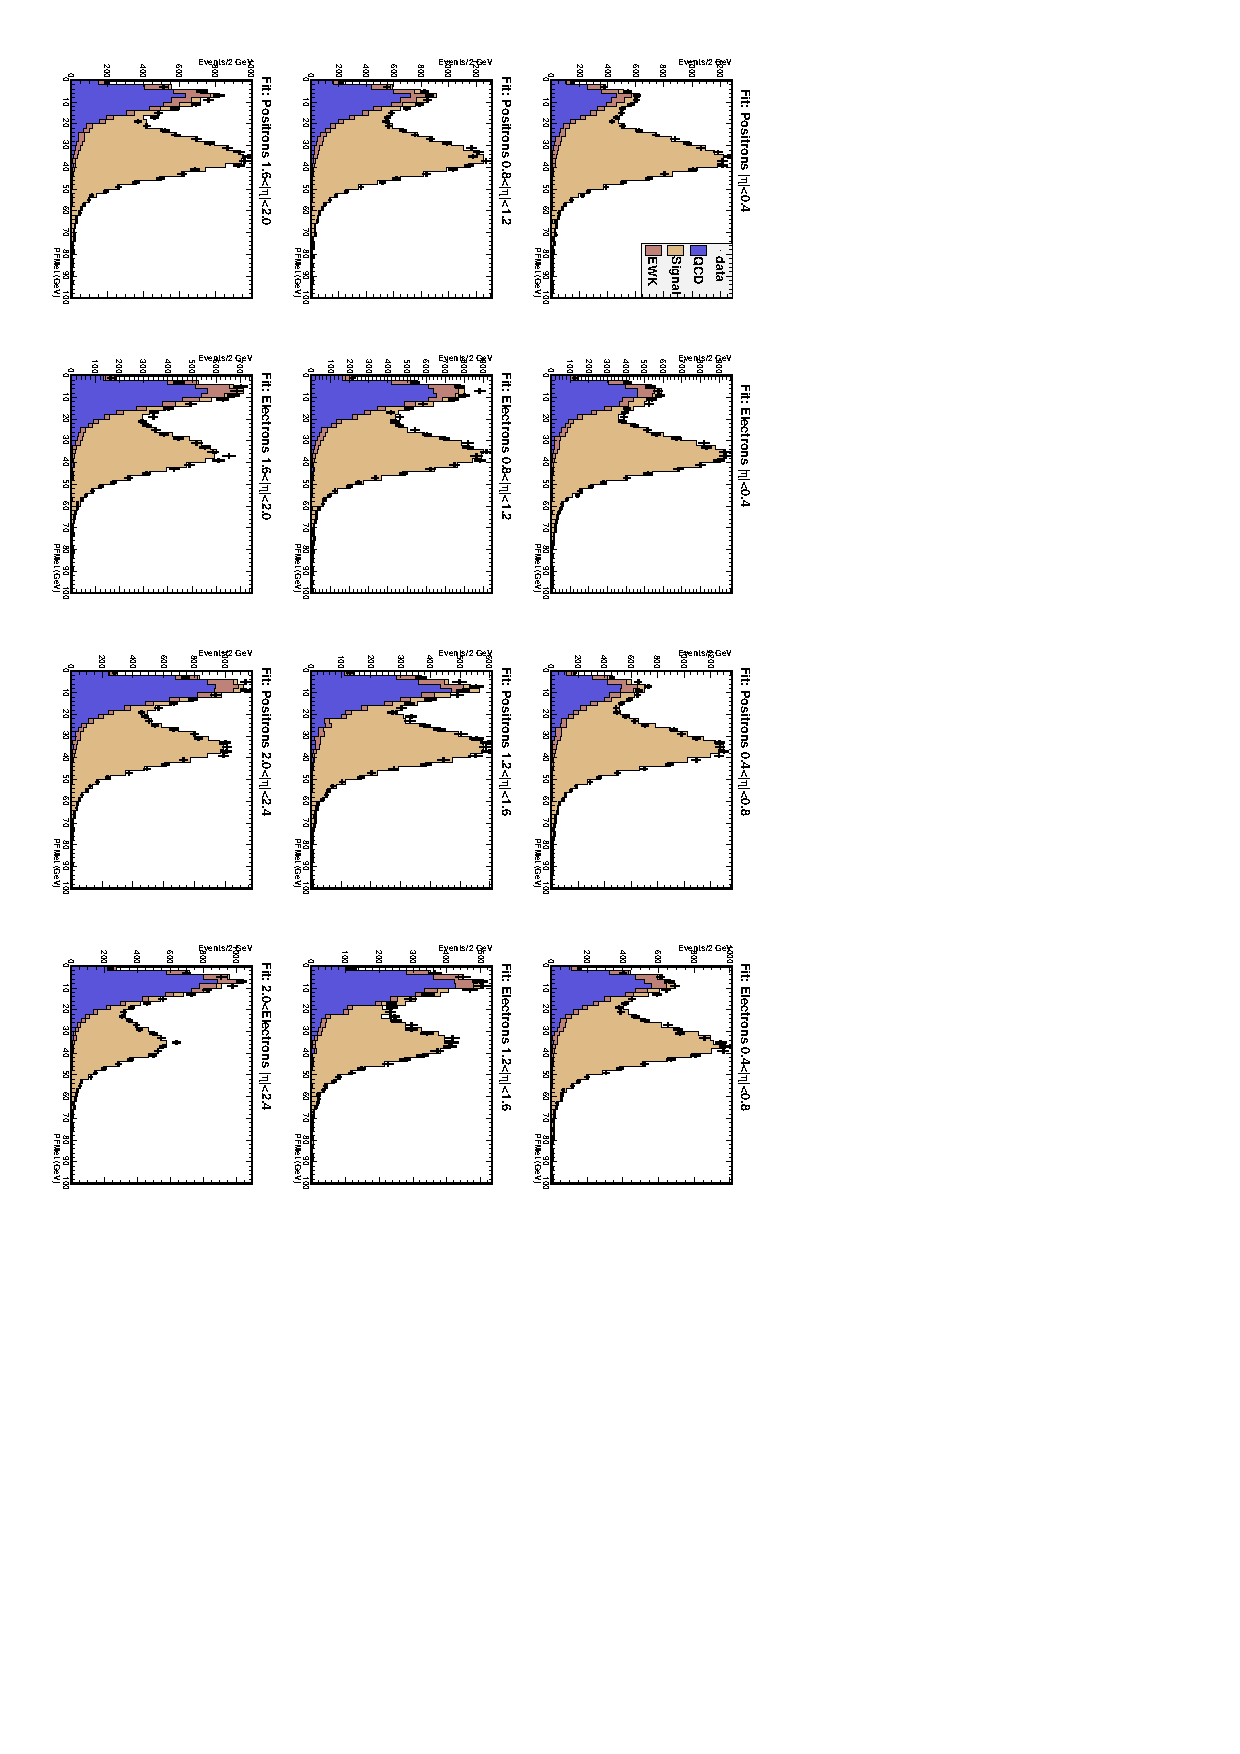
\includegraphics[trim = 80mm 0mm 0mm 100mm, clip, angle=90, width=0.95\textwidth]{Dec22_data}
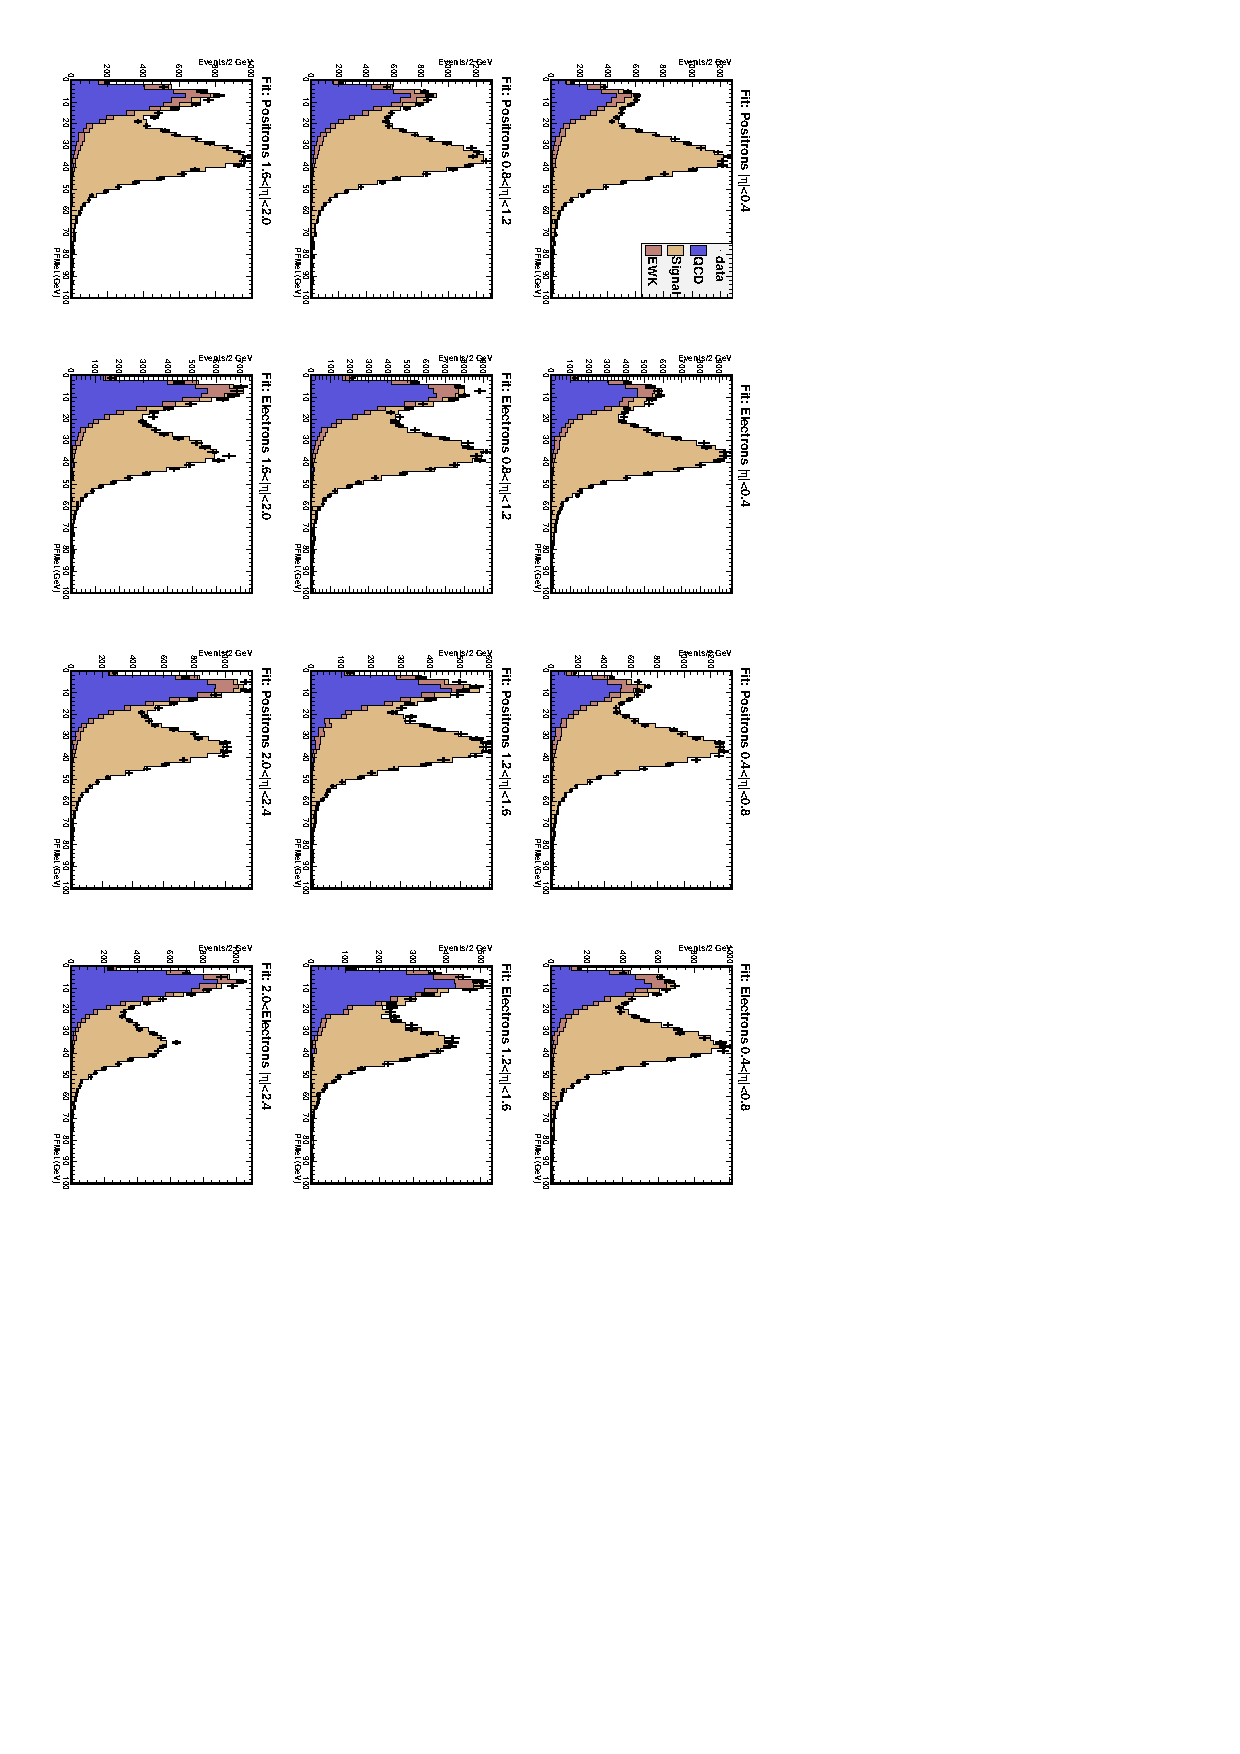
\includegraphics[trim = 40mm 100mm 40mm 0mm, clip, angle=90, width=0.95\textwidth]{Dec22_data}
\caption[The fit to \ETm for each pseudorapidity/charge bin.] {\label{fig:fit1}
The fit to \ETm\ for each pseudorapidity/charge bin.  The $x$-axis is the
particle flow \ETm (GeV) and the $y$-axis is the number of events
($2\GeV^{-1}$).}
\end{center}
\end{figure}

\begin{figure}
\begin{center}
% bottom right top left
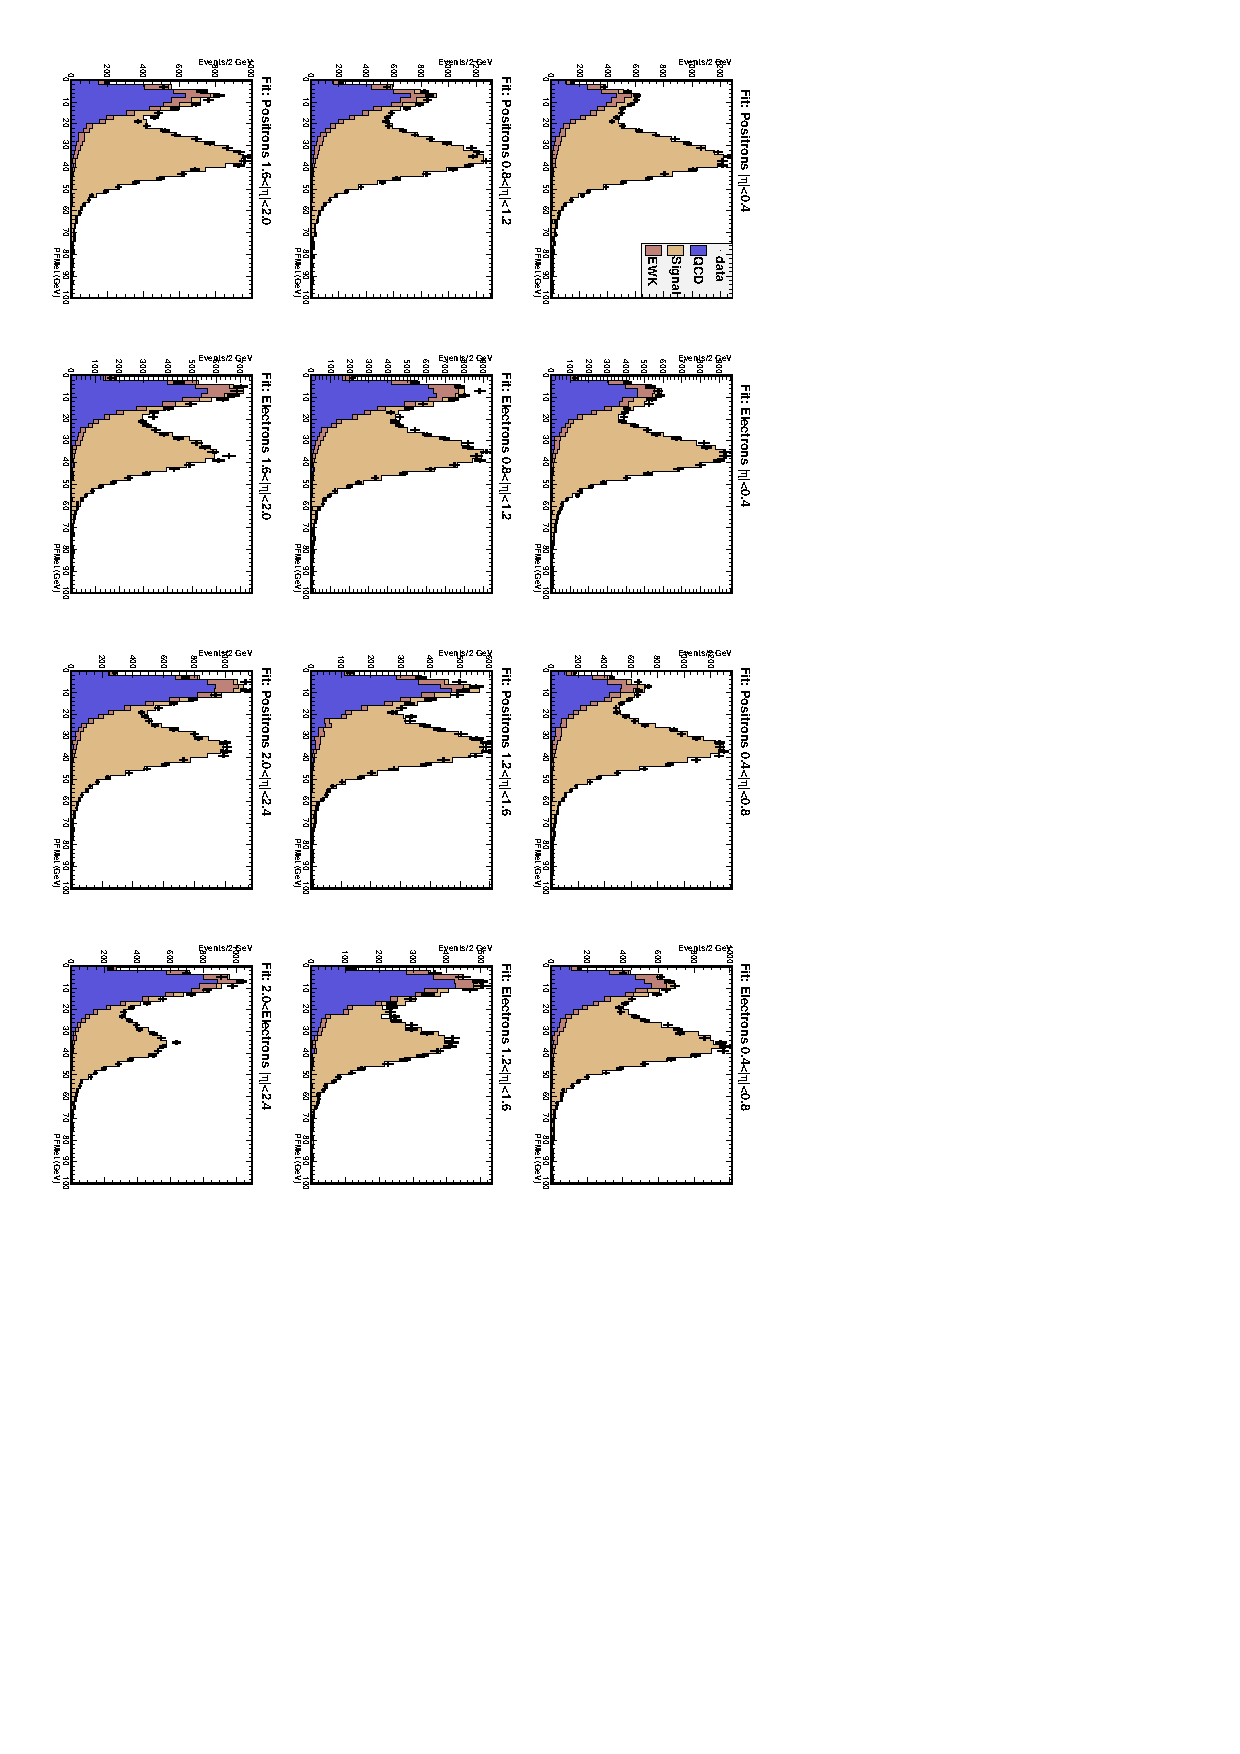
\includegraphics[trim = 40mm 0mm 40mm 100mm, clip, angle=90, width=0.95\textwidth]{Dec22_data}
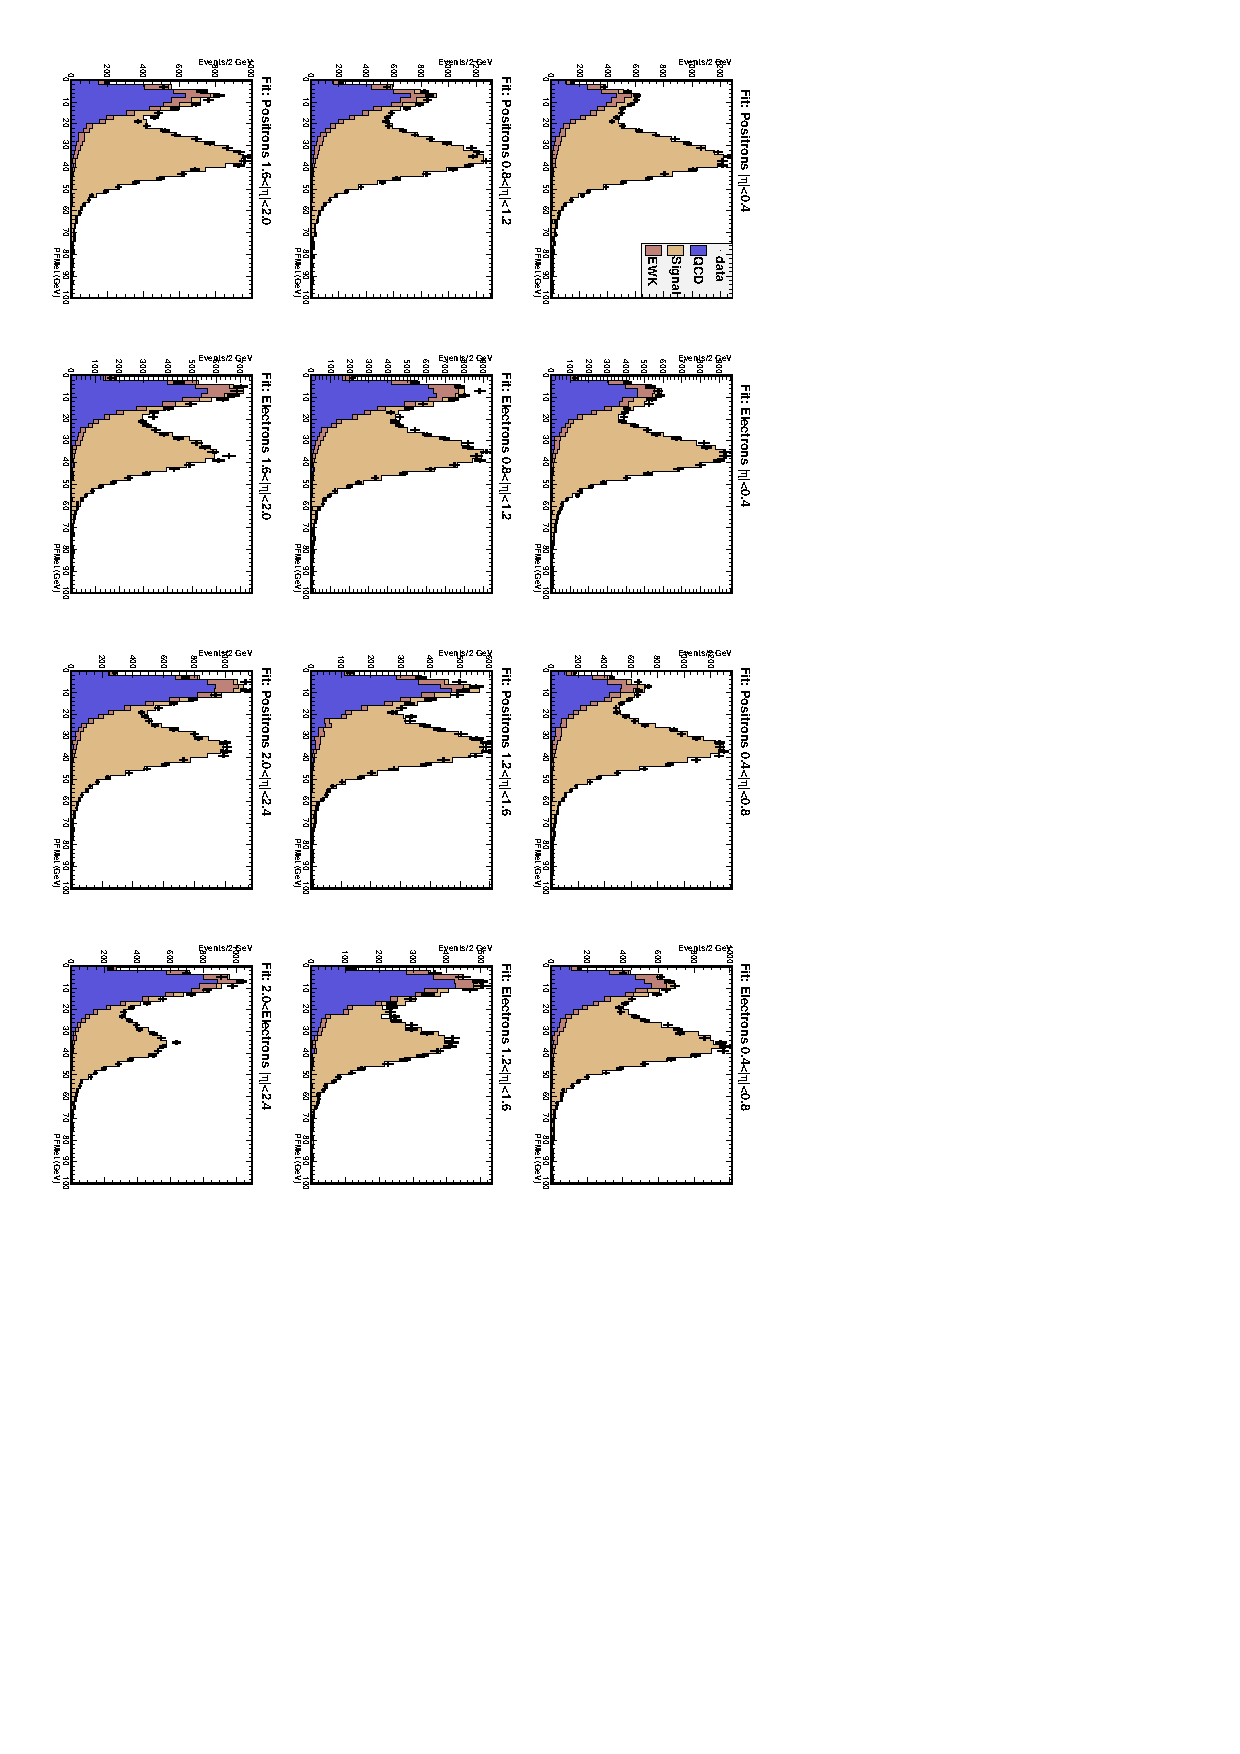
\includegraphics[trim = 0mm 100mm 80mm 0mm, clip, angle=90, width=0.95\textwidth]{Dec22_data}
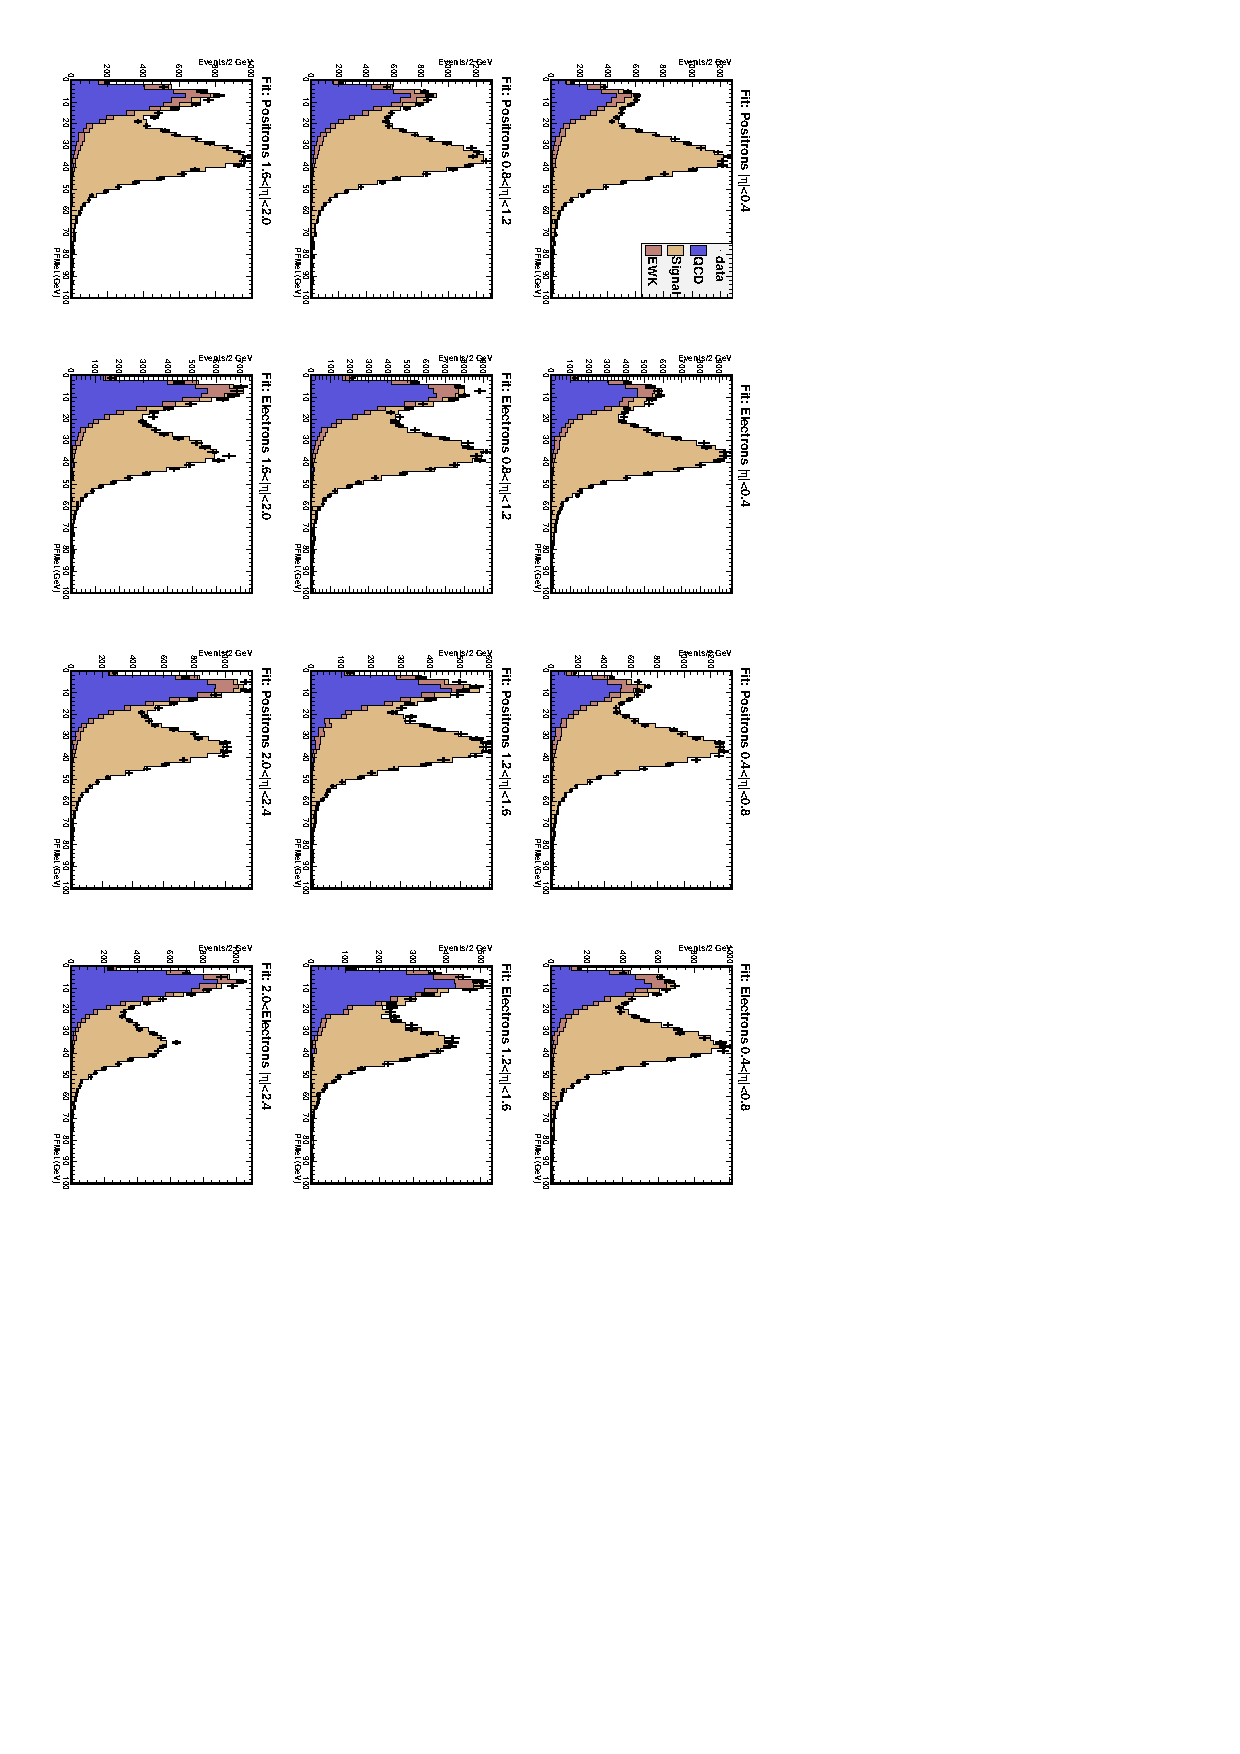
\includegraphics[trim = 0mm 0mm 80mm 100mm, clip, angle=90, width=0.95\textwidth]{Dec22_data}
\caption[The fit to \ETm\ for each pseudorapidity/charge bin.]
{\label{fig:fit2} The fit to \ETm\ for each pseudorapidity/charge
bin.  The $x$-axis is the particle flow \ETm (GeV) and the $y$-axis is the
number of events ($2\GeV^{-1}$).}
\end{center}
\end{figure}

%\begin{figure}
%\begin{center}
% bottom right top left
%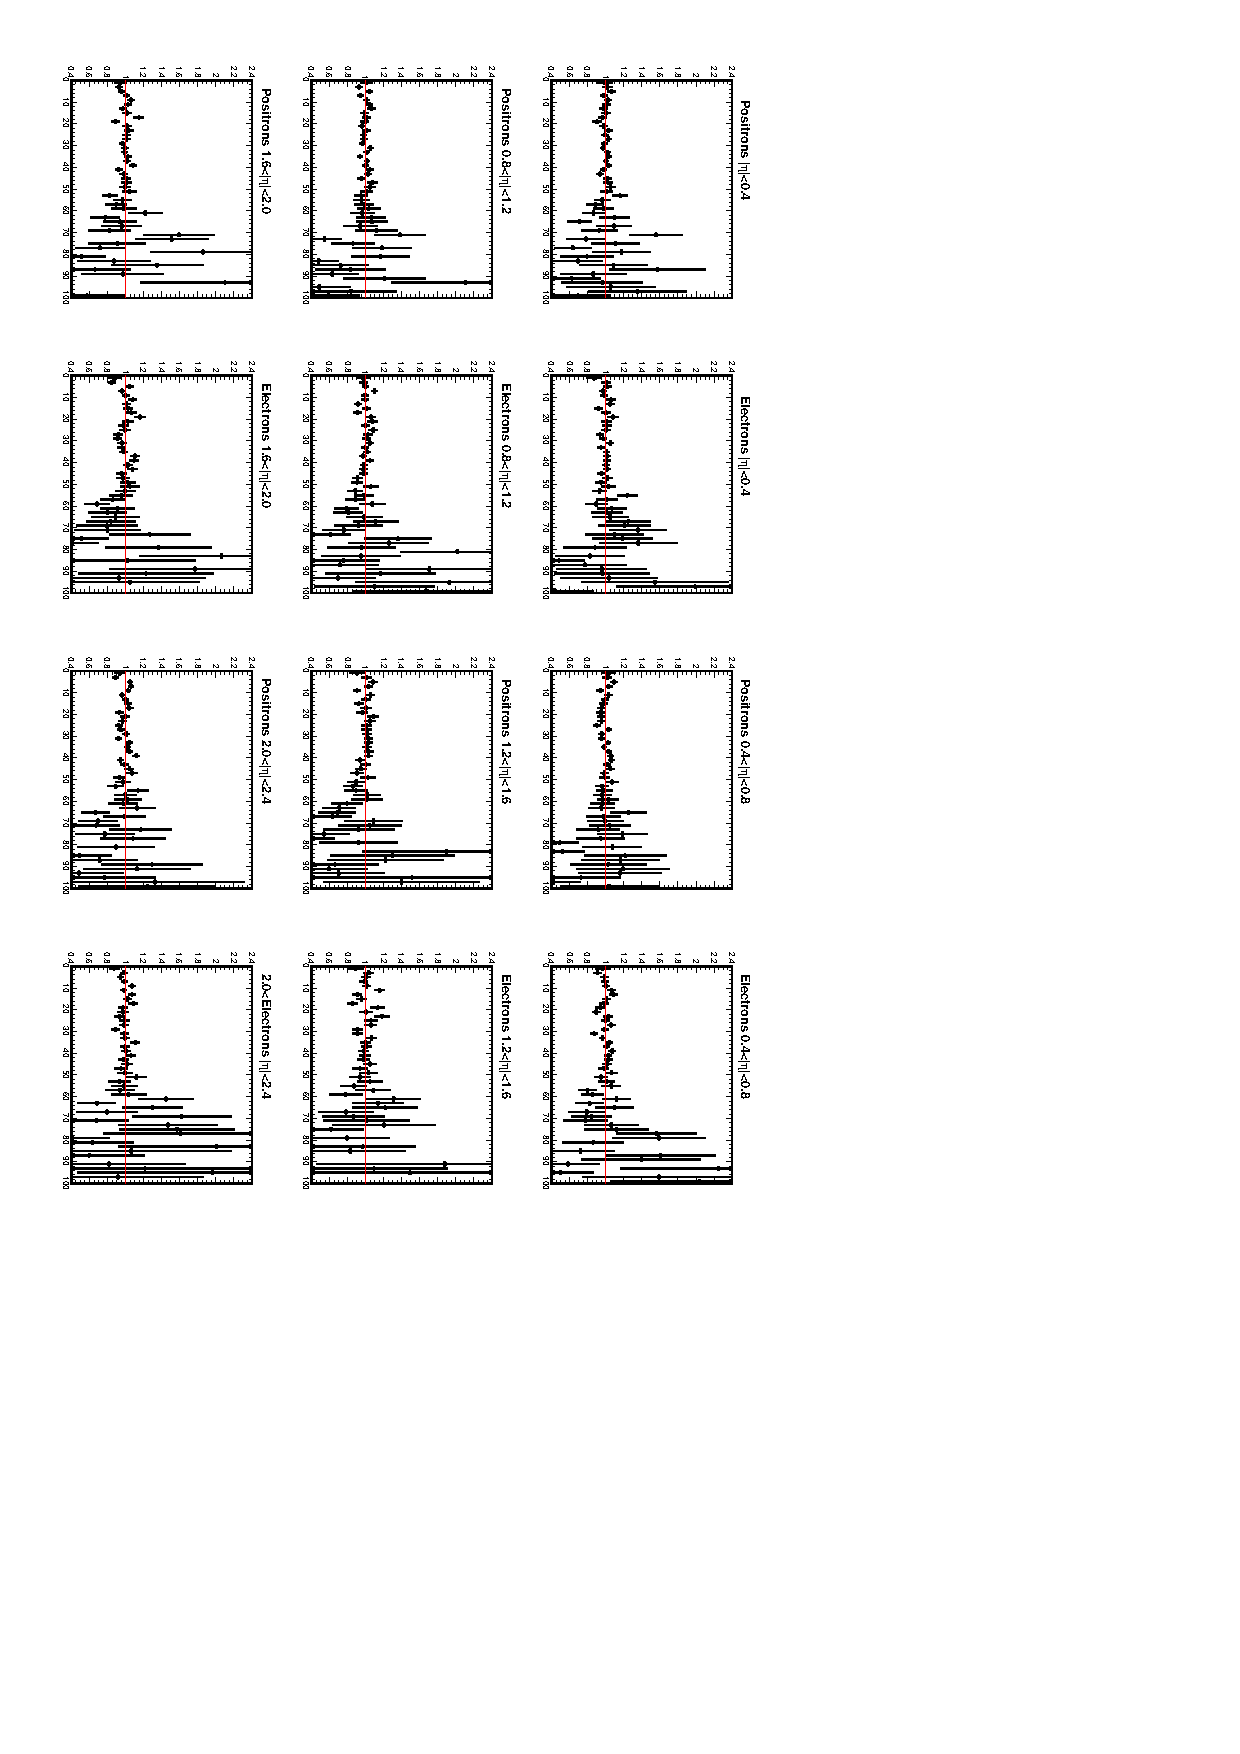
\includegraphics[trim = 80mm 100mm 0mm 0mm, clip, angle=90, width=0.95\textwidth]{Dec22_fitratio}
%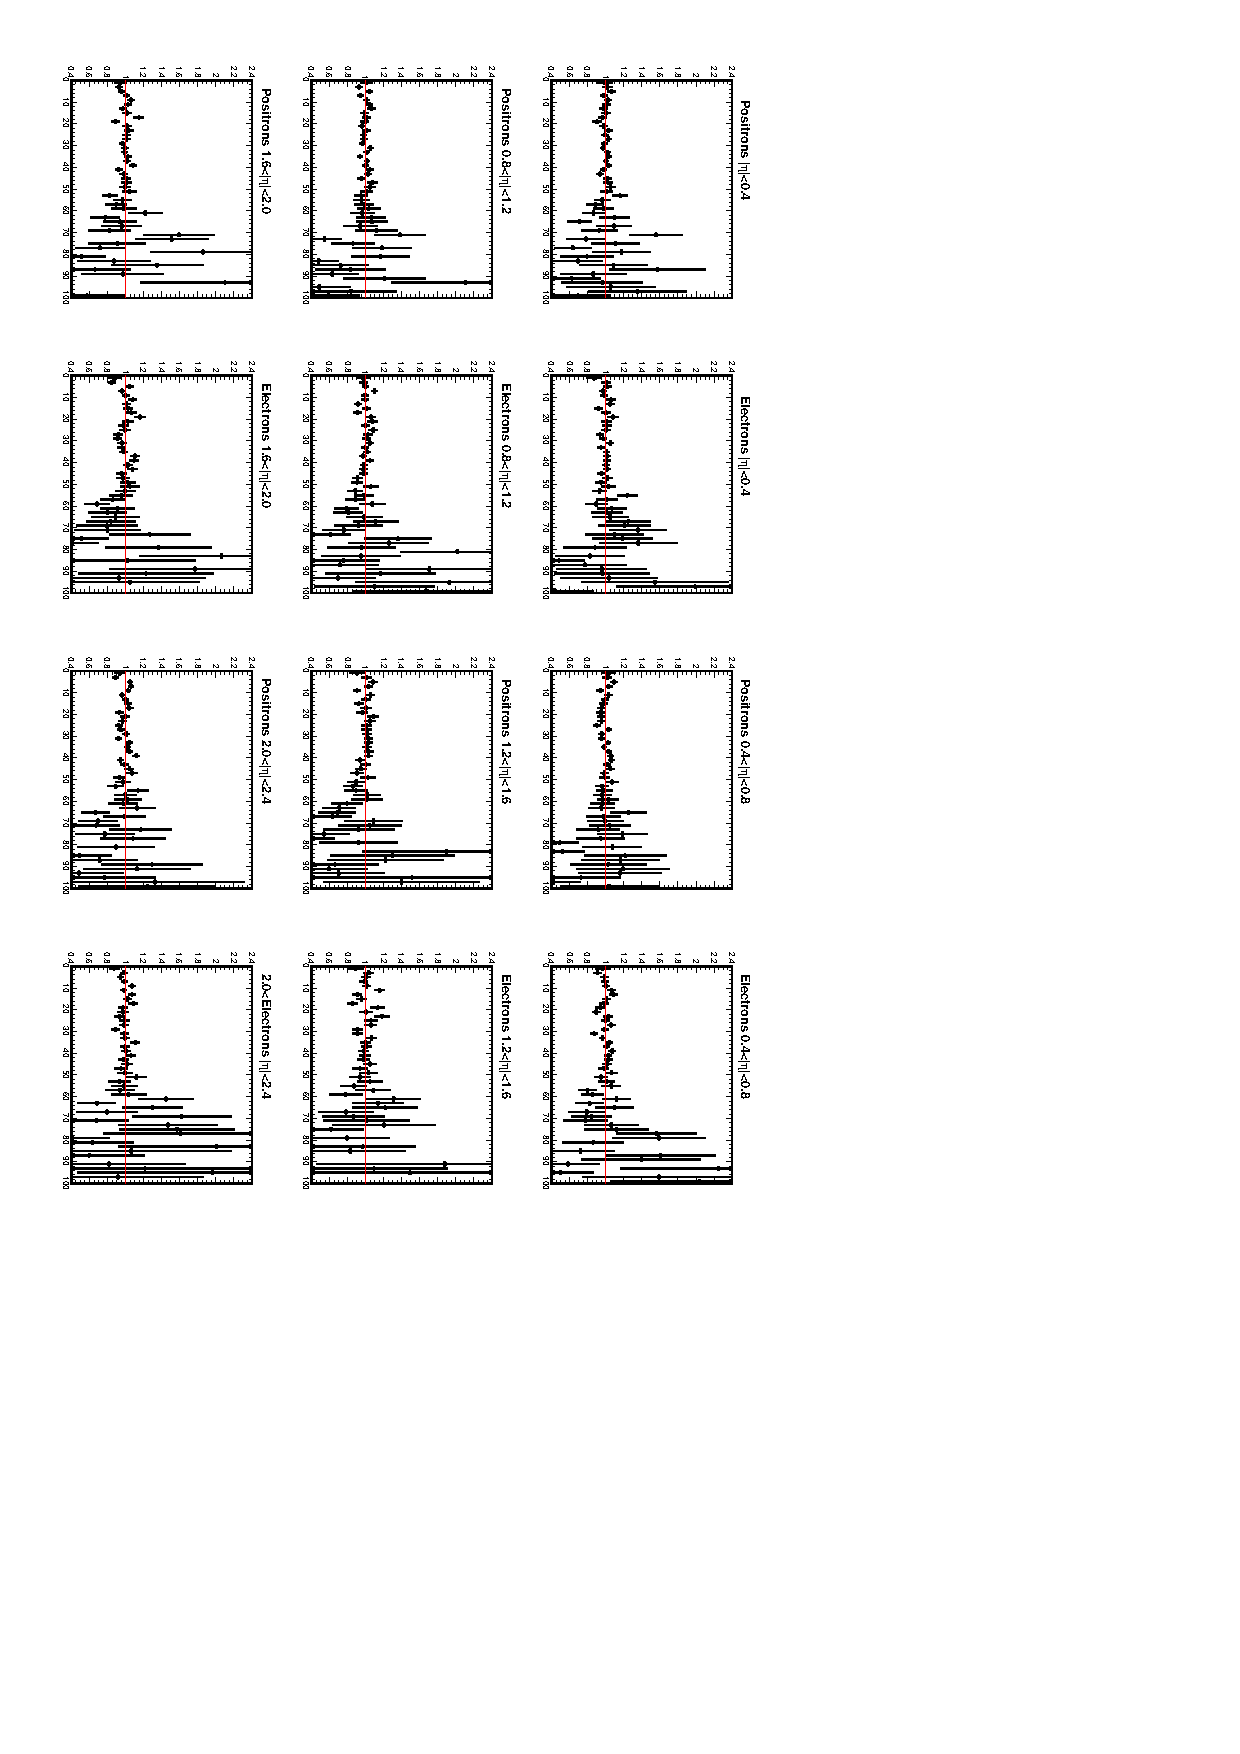
\includegraphics[trim = 80mm 0mm 0mm 100mm, clip, angle=90, width=0.95\textwidth]{Dec22_fitratio}
%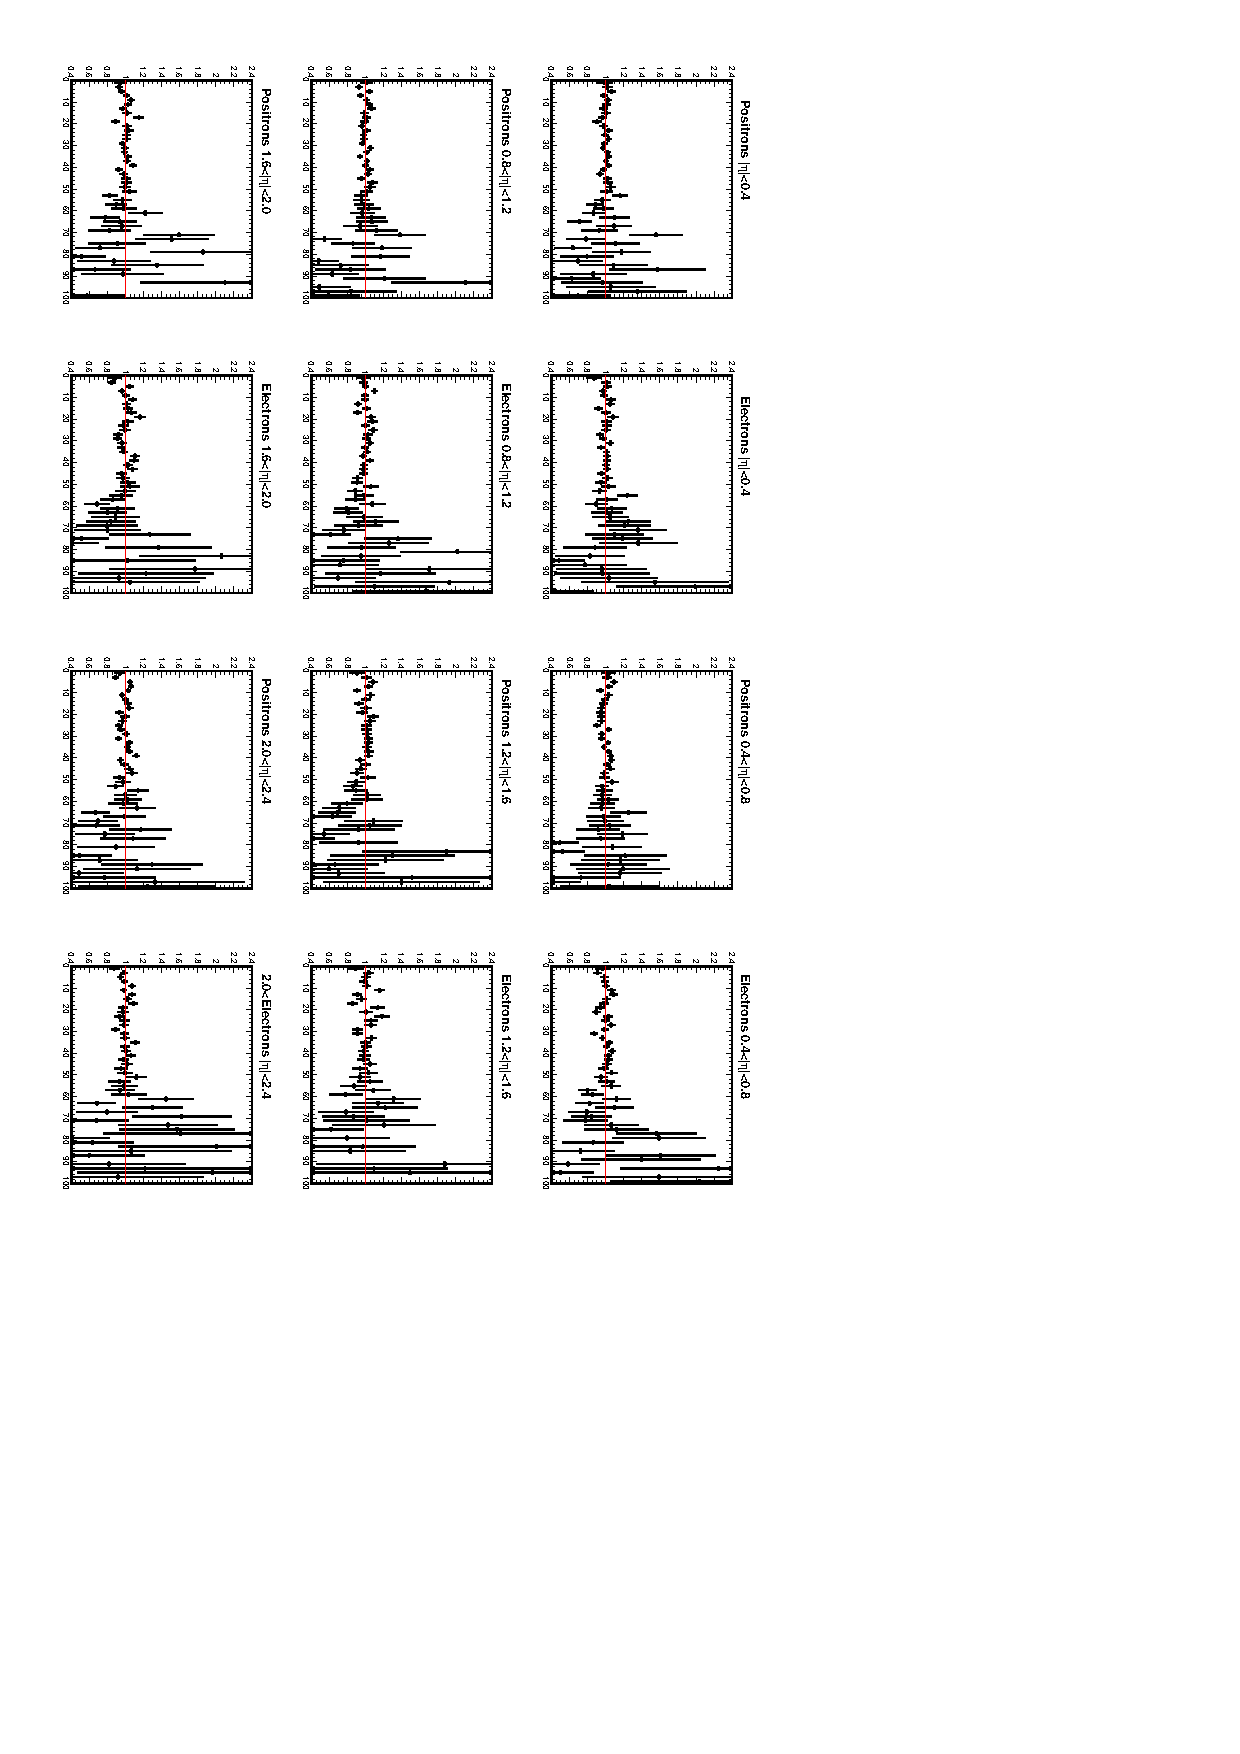
\includegraphics[trim = 40mm 100mm 40mm 0mm, clip, angle=90, width=0.95\textwidth]{Dec22_fitratio}
%\caption{\label{fig:fit1ratio}Ratio between fit and data for each pseudorapidity/charge bin.
%The $x$-axis is the particle flow \ETm (GeV).}
%\end{center}
%\end{figure}

%\begin{figure}
%\begin{center}
%% bottom right top left
%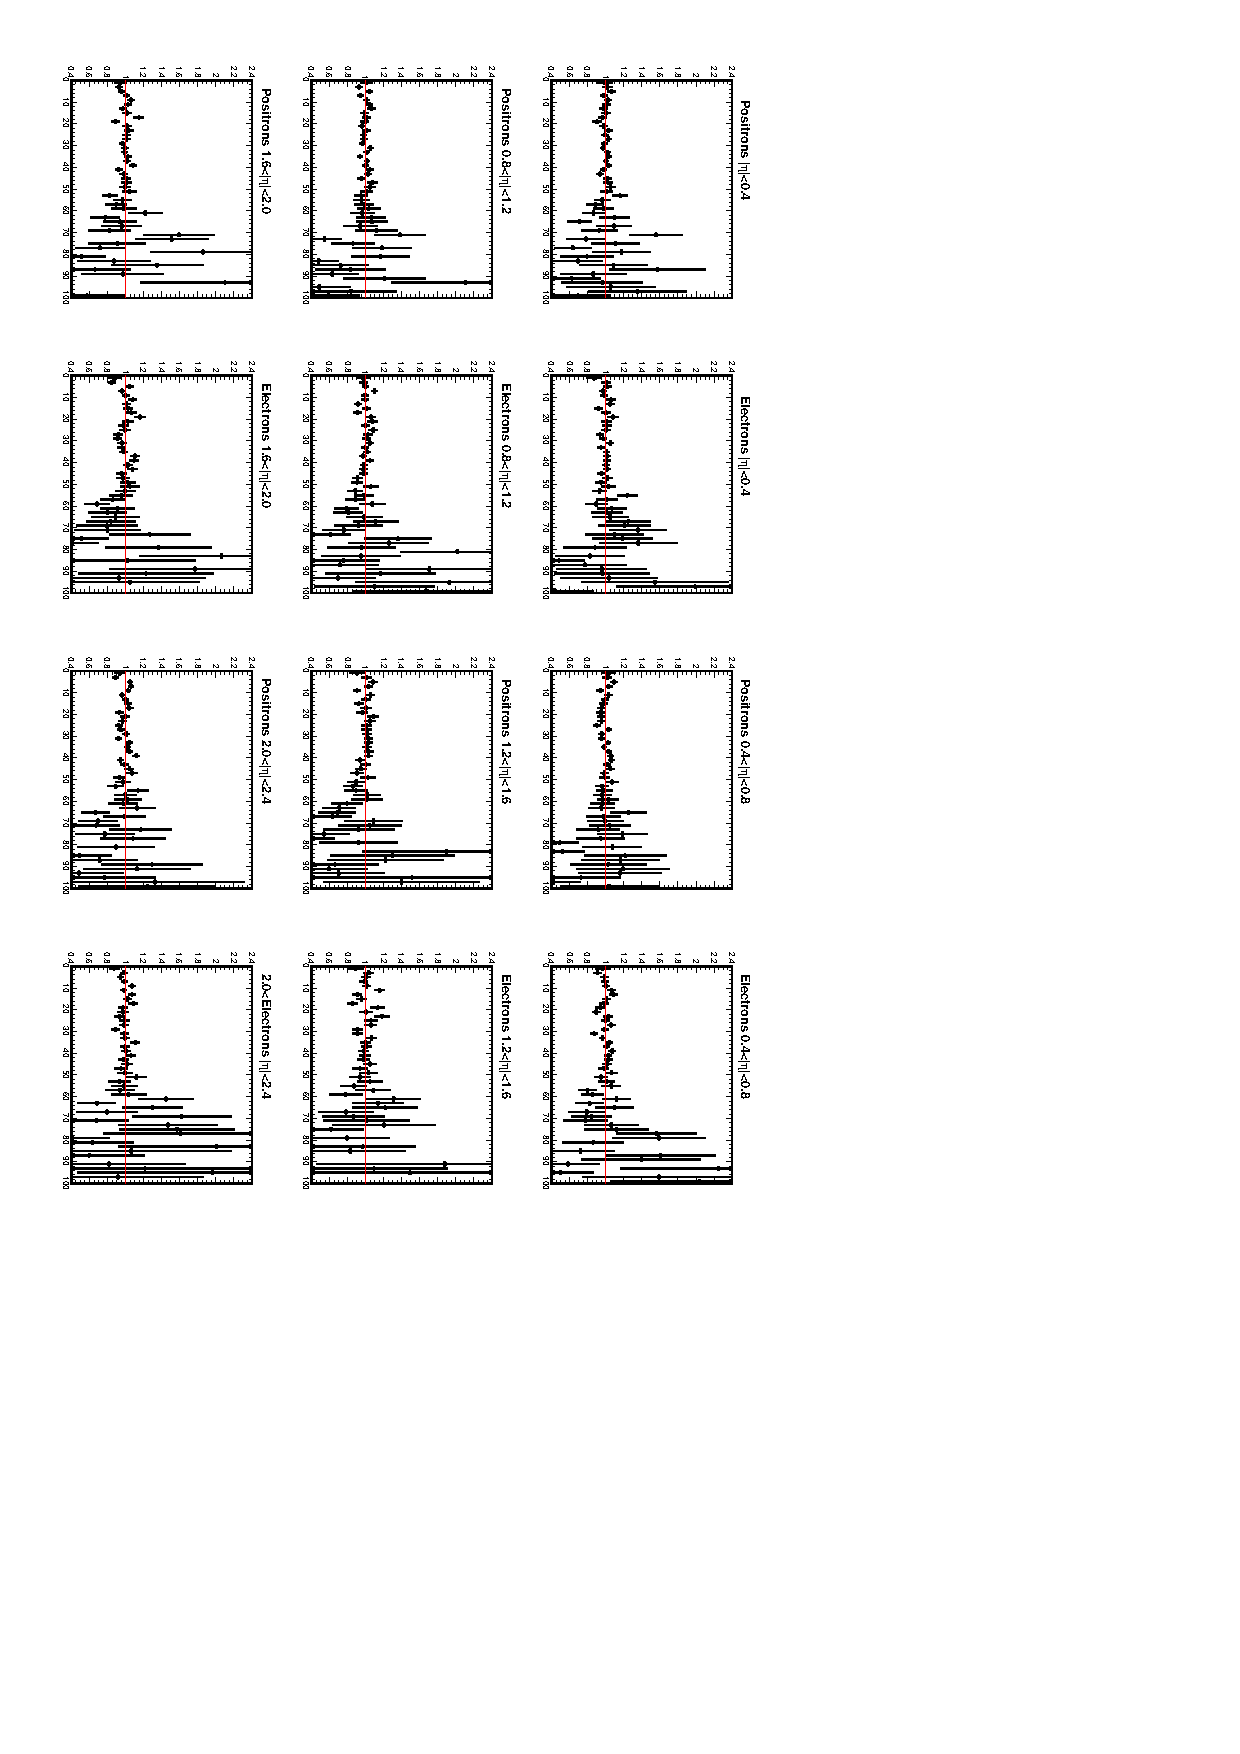
\includegraphics[trim = 40mm 0mm 40mm 100mm, clip, angle=90, width=0.95\textwidth]{Dec22_fitratio}
%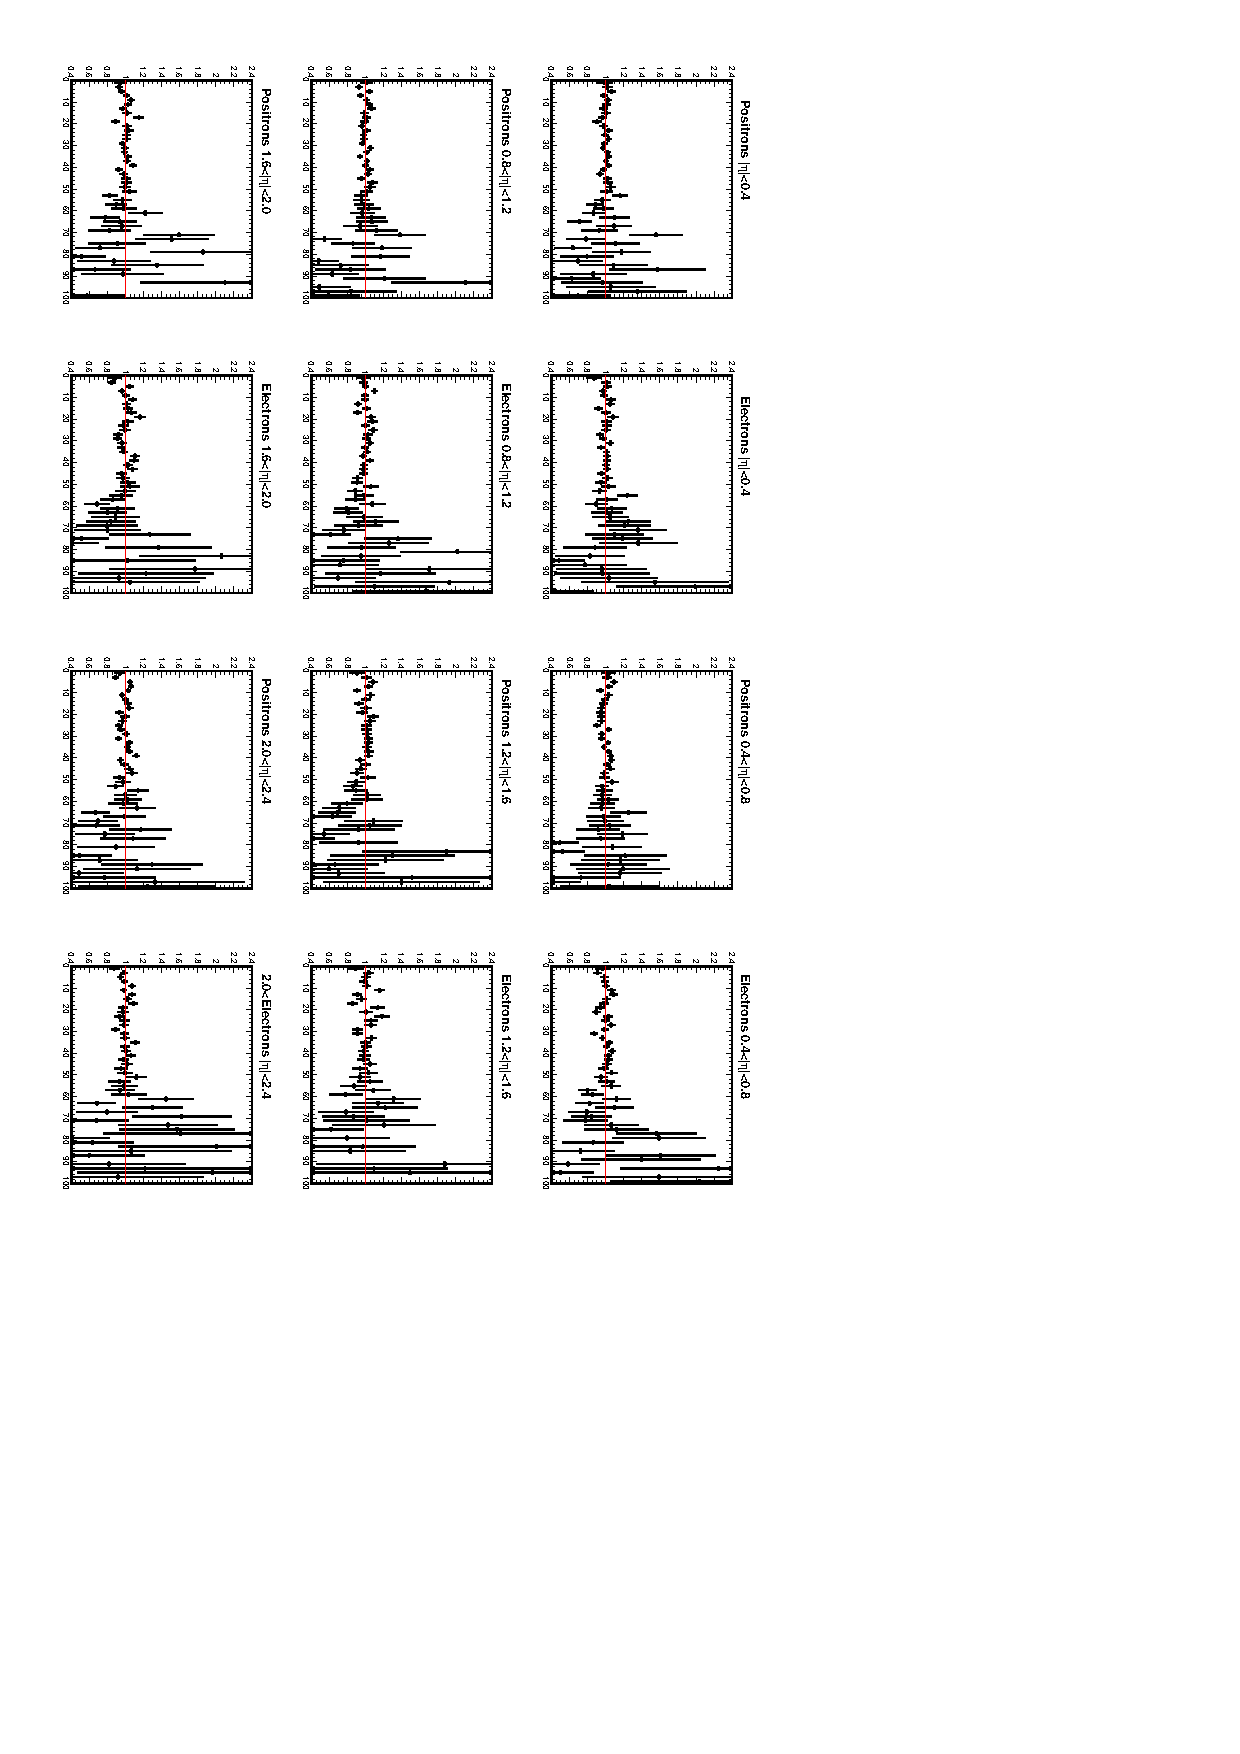
\includegraphics[trim = 0mm 100mm 80mm 0mm, clip, angle=90, width=0.95\textwidth]{Dec22_fitratio}
%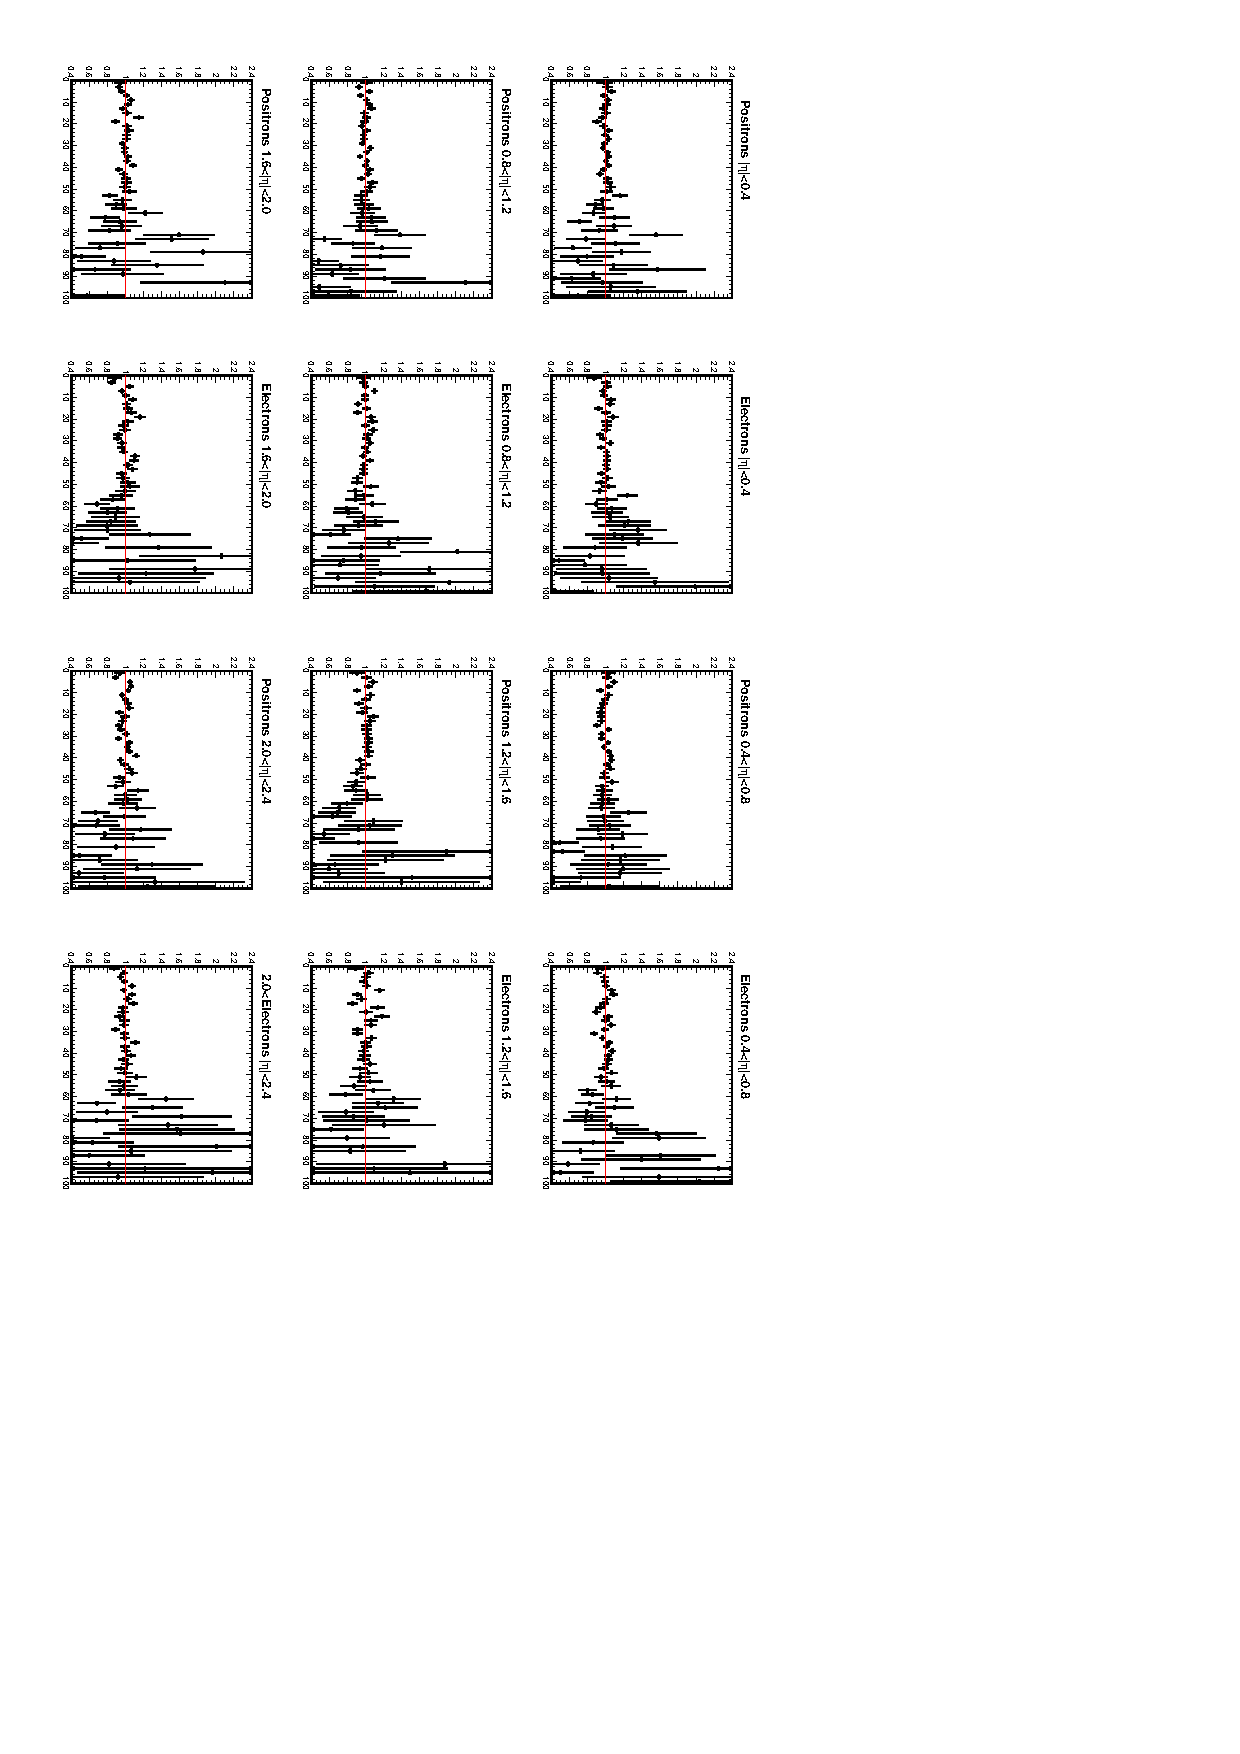
\includegraphics[trim = 0mm 0mm 80mm 100mm, clip, angle=90, width=0.95\textwidth]{Dec22_fitratio}
%\caption{\label{fig:fit2ratio}Ratio between fit and data for each
%pseudorapidity/charge bin.  The $x$-axis is the particle flow \ETm (GeV).}
%\end{center}
%\end{figure}

\clearpage

\section{\unit{840}{\invpb}}

\begin{figure}
\begin{center}
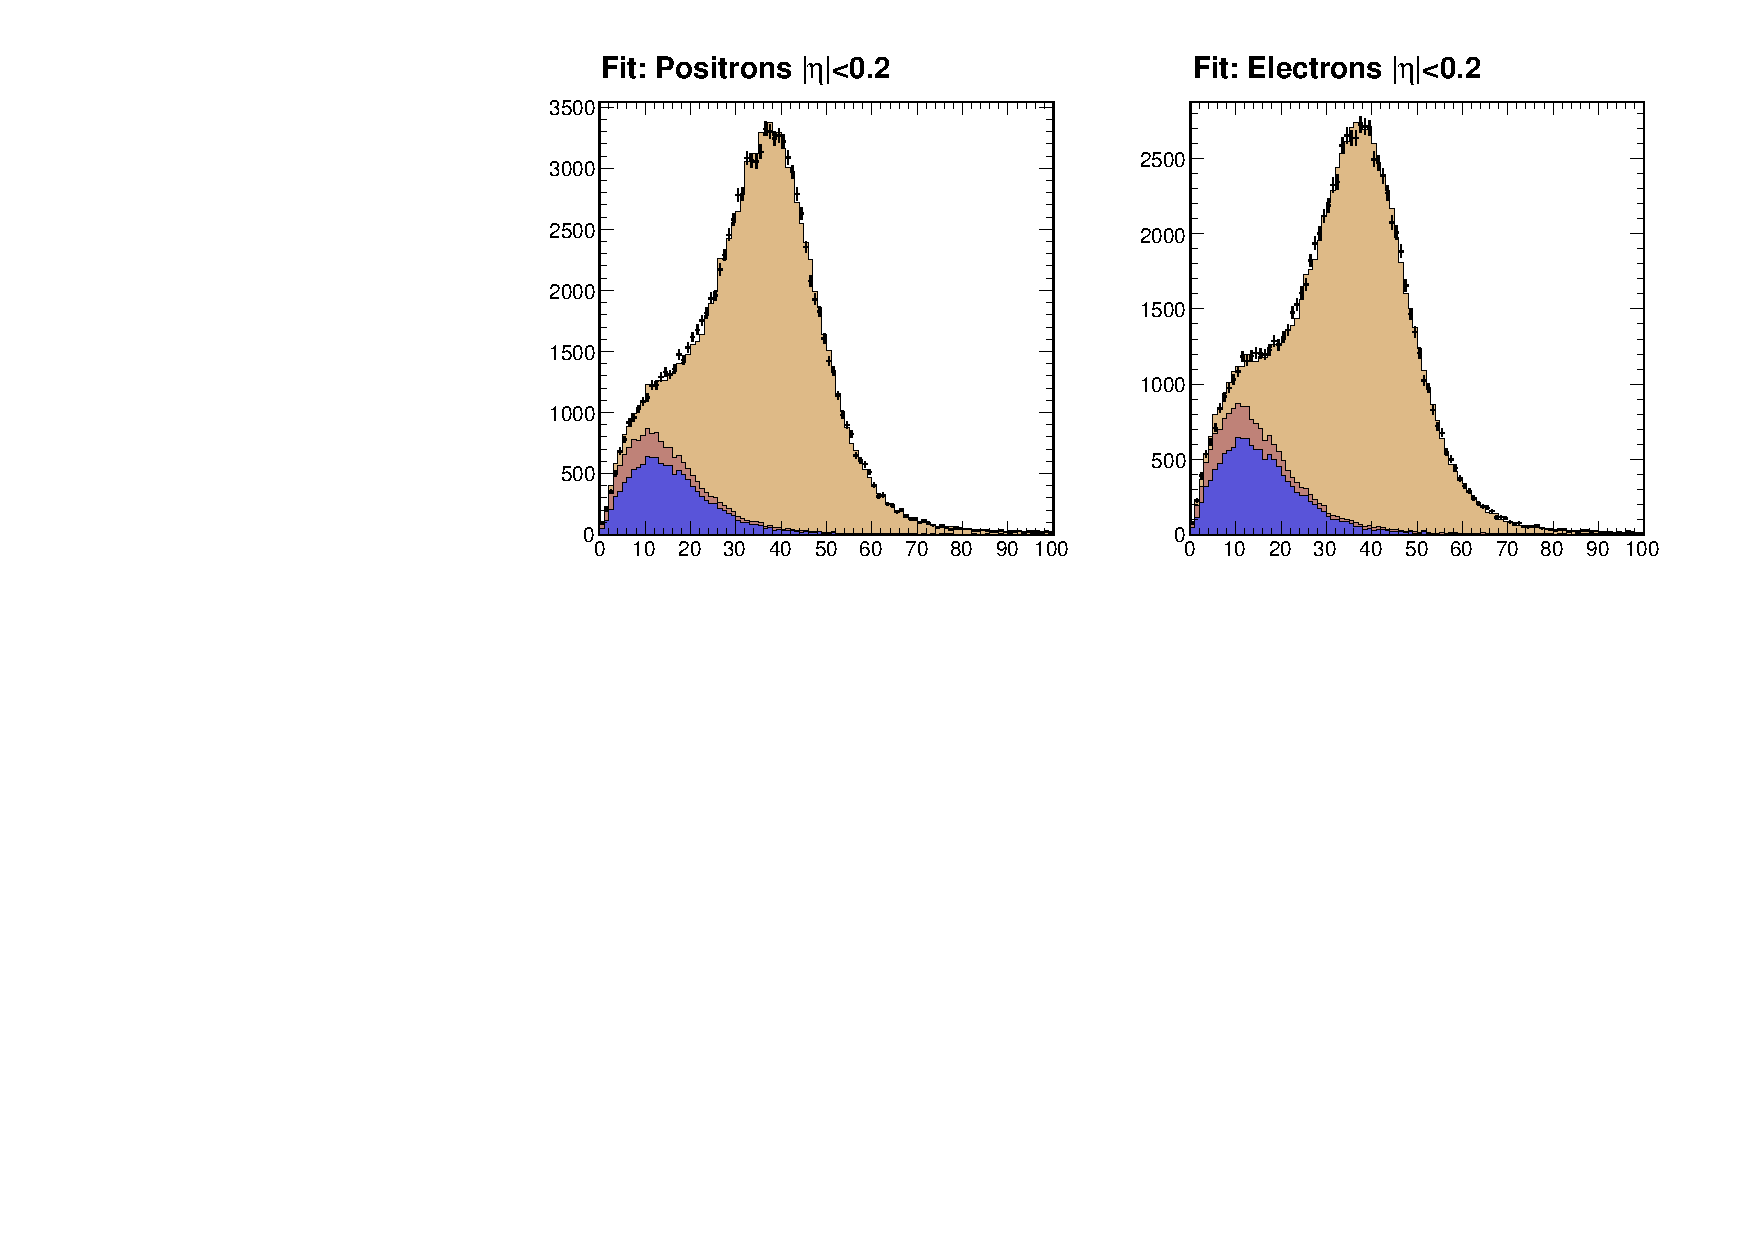
\includegraphics[width=0.95\textwidth]{data_0.pdf} \\
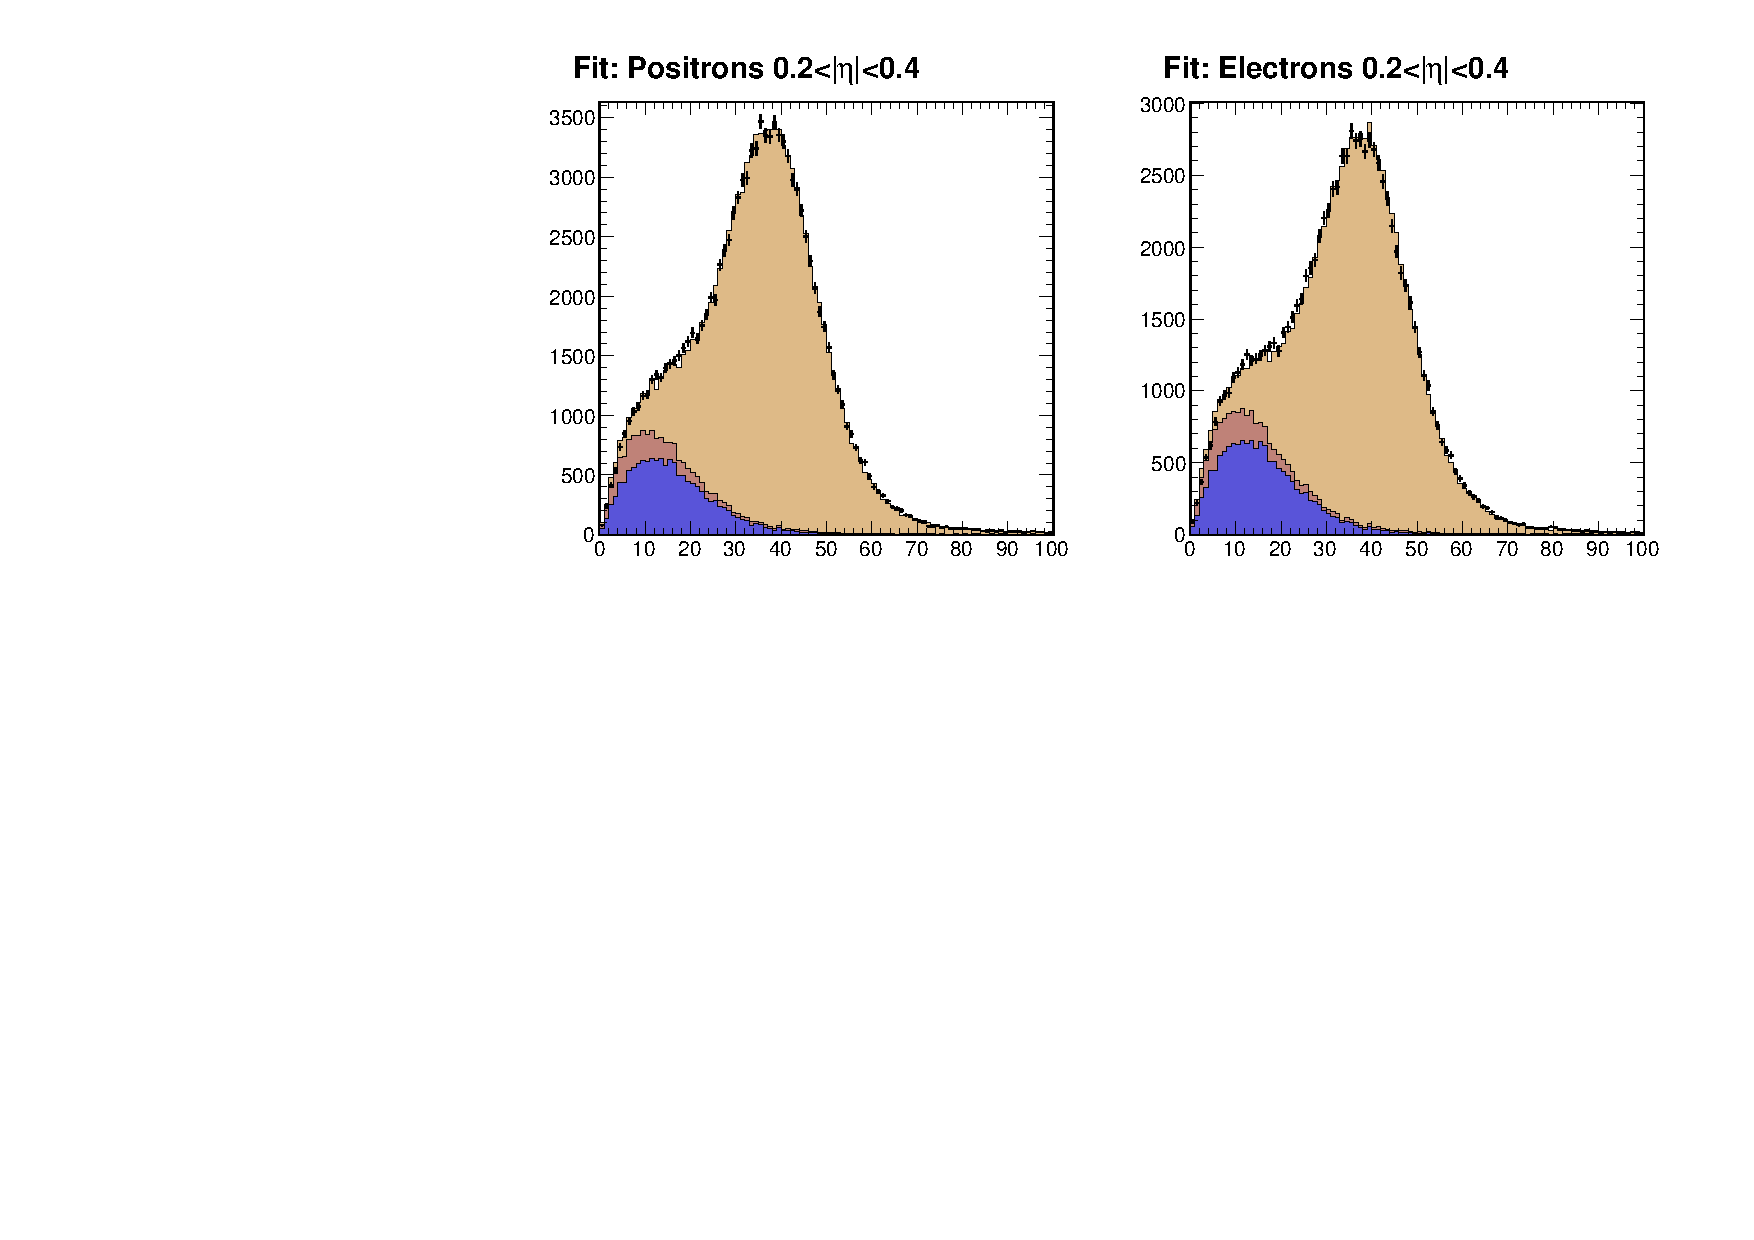
\includegraphics[width=0.95\textwidth]{data_1.pdf} \\
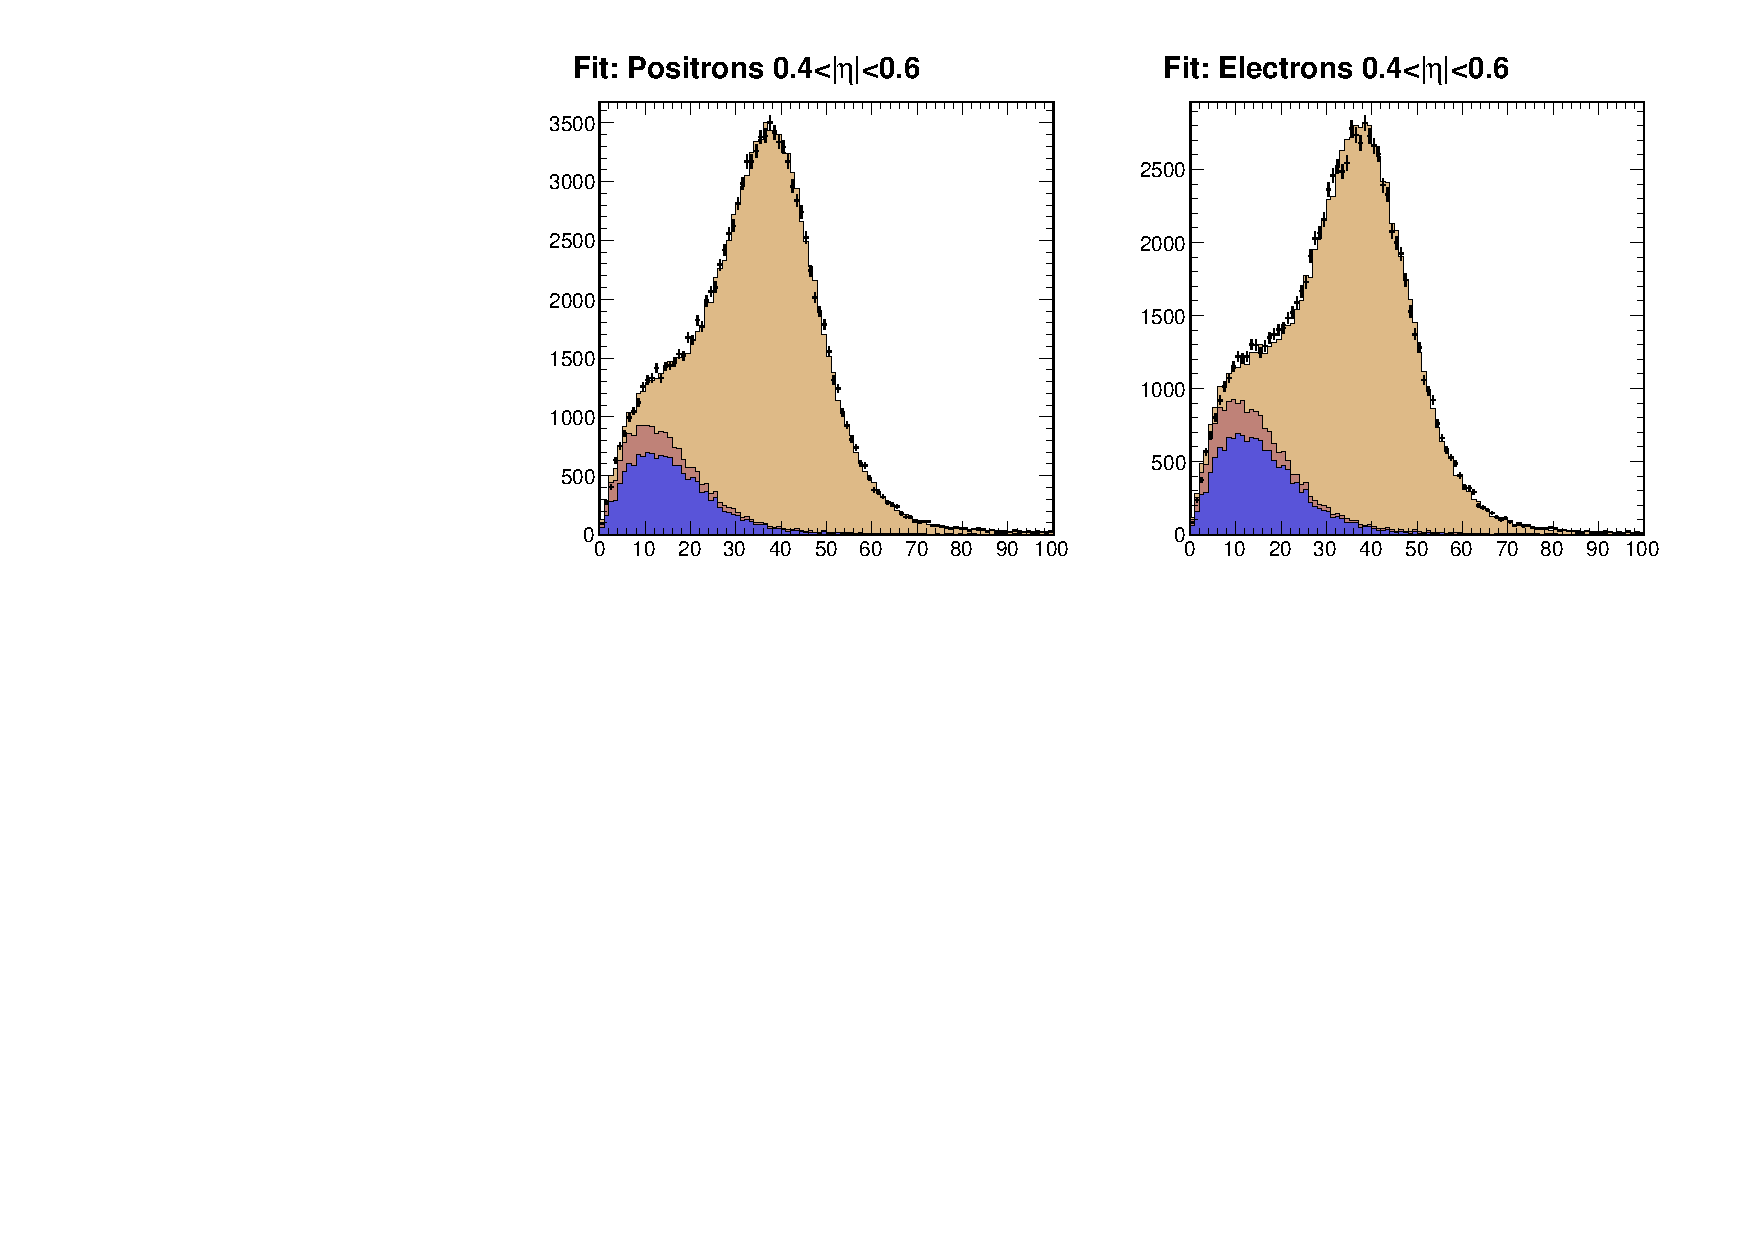
\includegraphics[width=0.95\textwidth]{data_2.pdf}
\caption[The fit to \MET for pseudorapidity bins 1,2 and 3.]
{\label{fig:data1} The fit to \MET\ for pseudorapidity bins 1,2 and
3.  The $x$-axis is the particle flow \ETm (GeV) and the $y$-axis is the number
of events ($\GeV^{-1}$).}
\end{center}
\end{figure}

\begin{figure}
\begin{center}
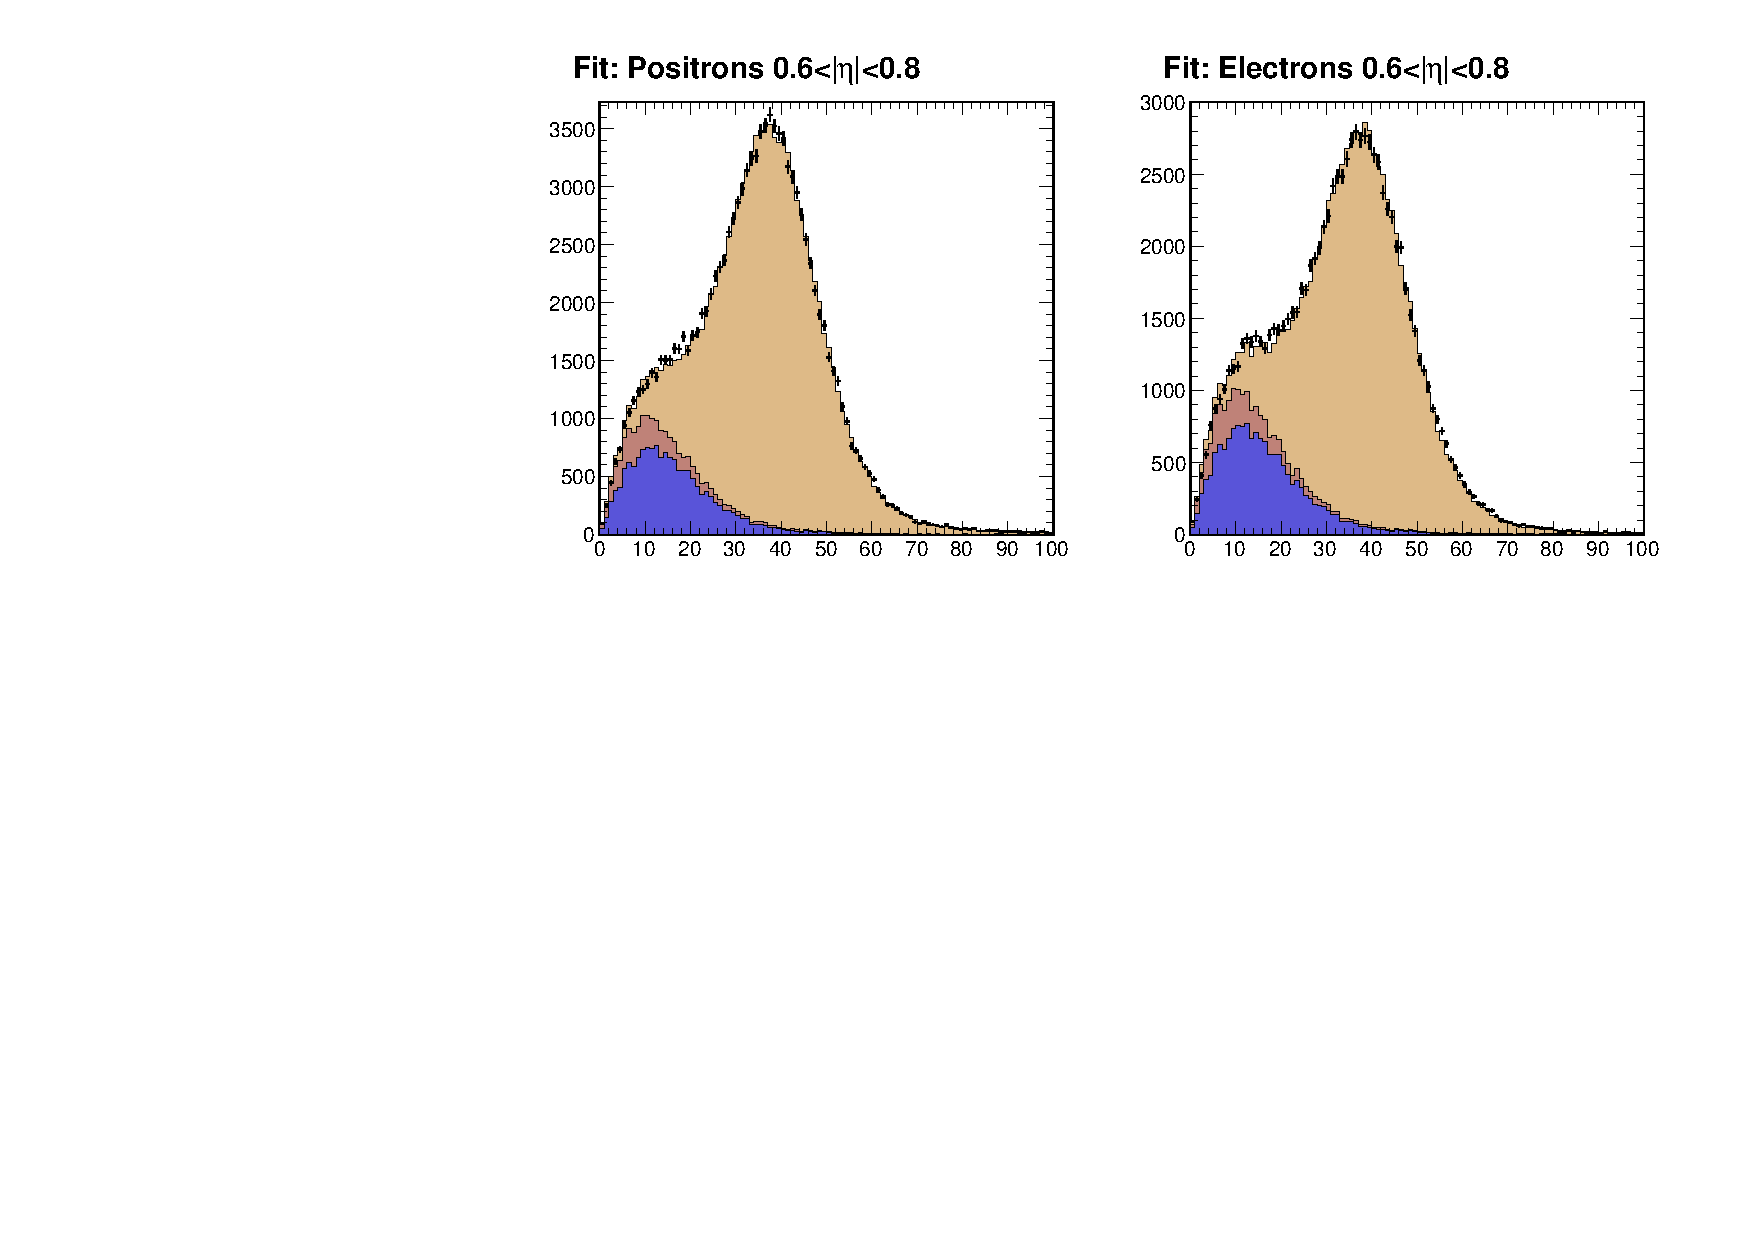
\includegraphics[width=0.95\textwidth]{data_3.pdf} \\
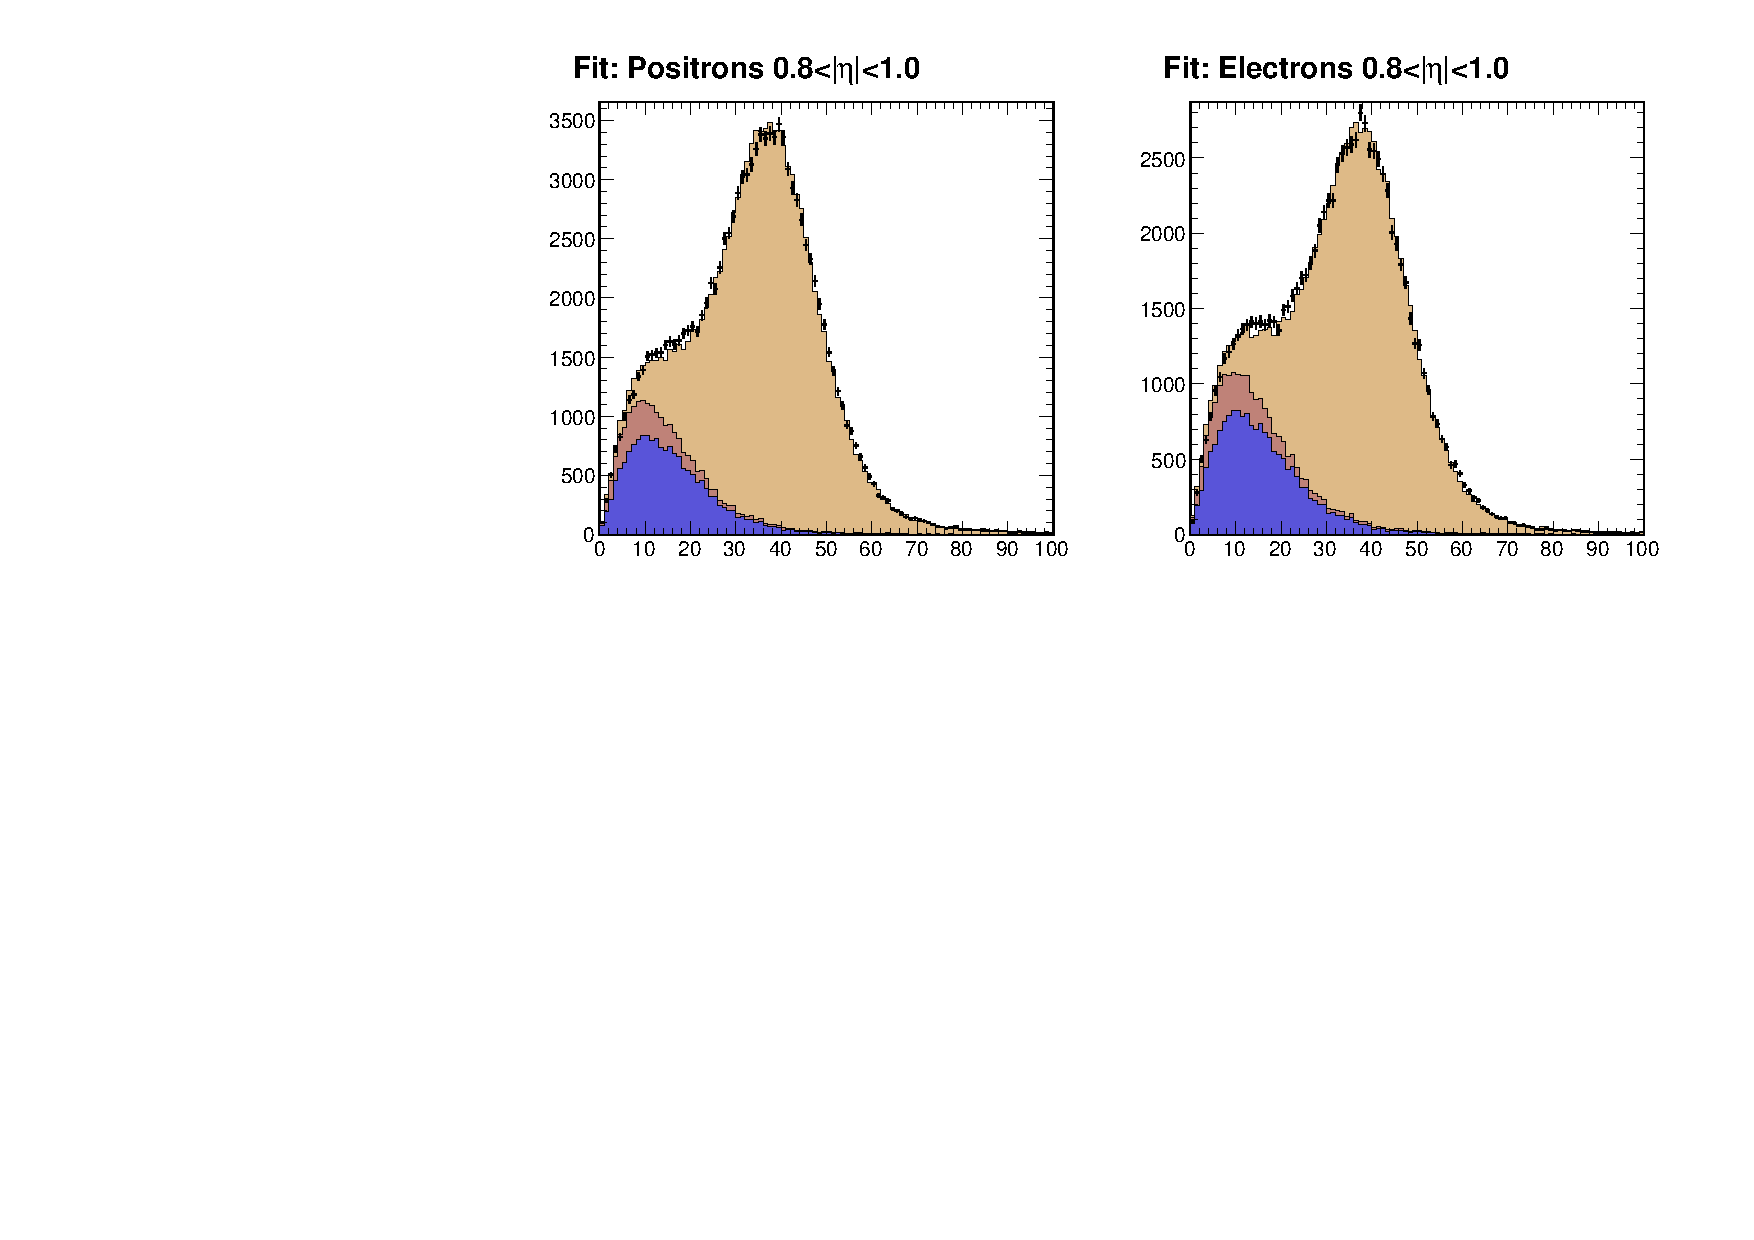
\includegraphics[width=0.95\textwidth]{data_4.pdf} \\
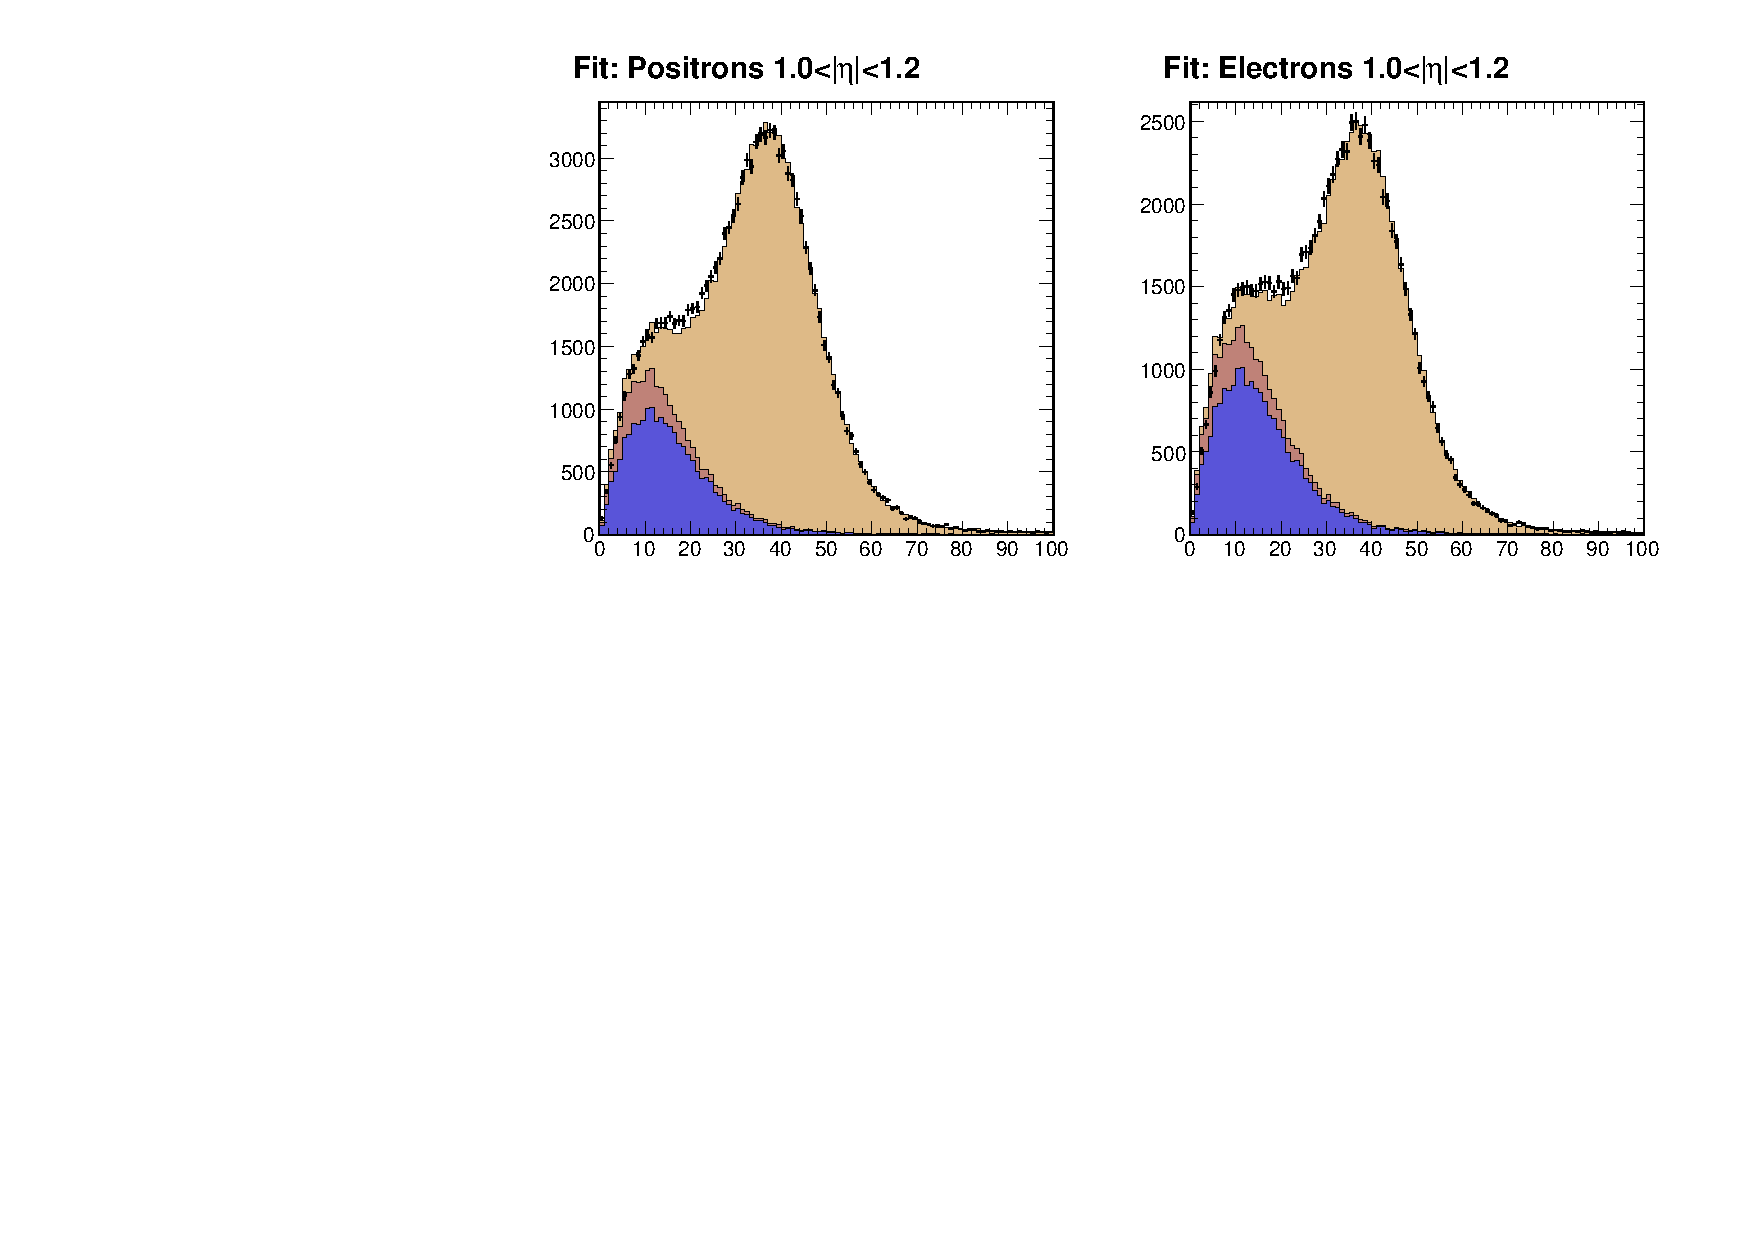
\includegraphics[width=0.95\textwidth]{data_5.pdf}
\caption[The fit to \MET for pseudorapidity bins 4,5 and 6.]
{\label{fig:data2} The fit to \MET\ for pseudorapidity bins 4,5 and
6.  The $x$-axis is the particle flow \ETm (GeV) and the $y$-axis is the number
of events ($\GeV^{-1}$).}
\end{center}
\end{figure}

\begin{figure}
\begin{center}
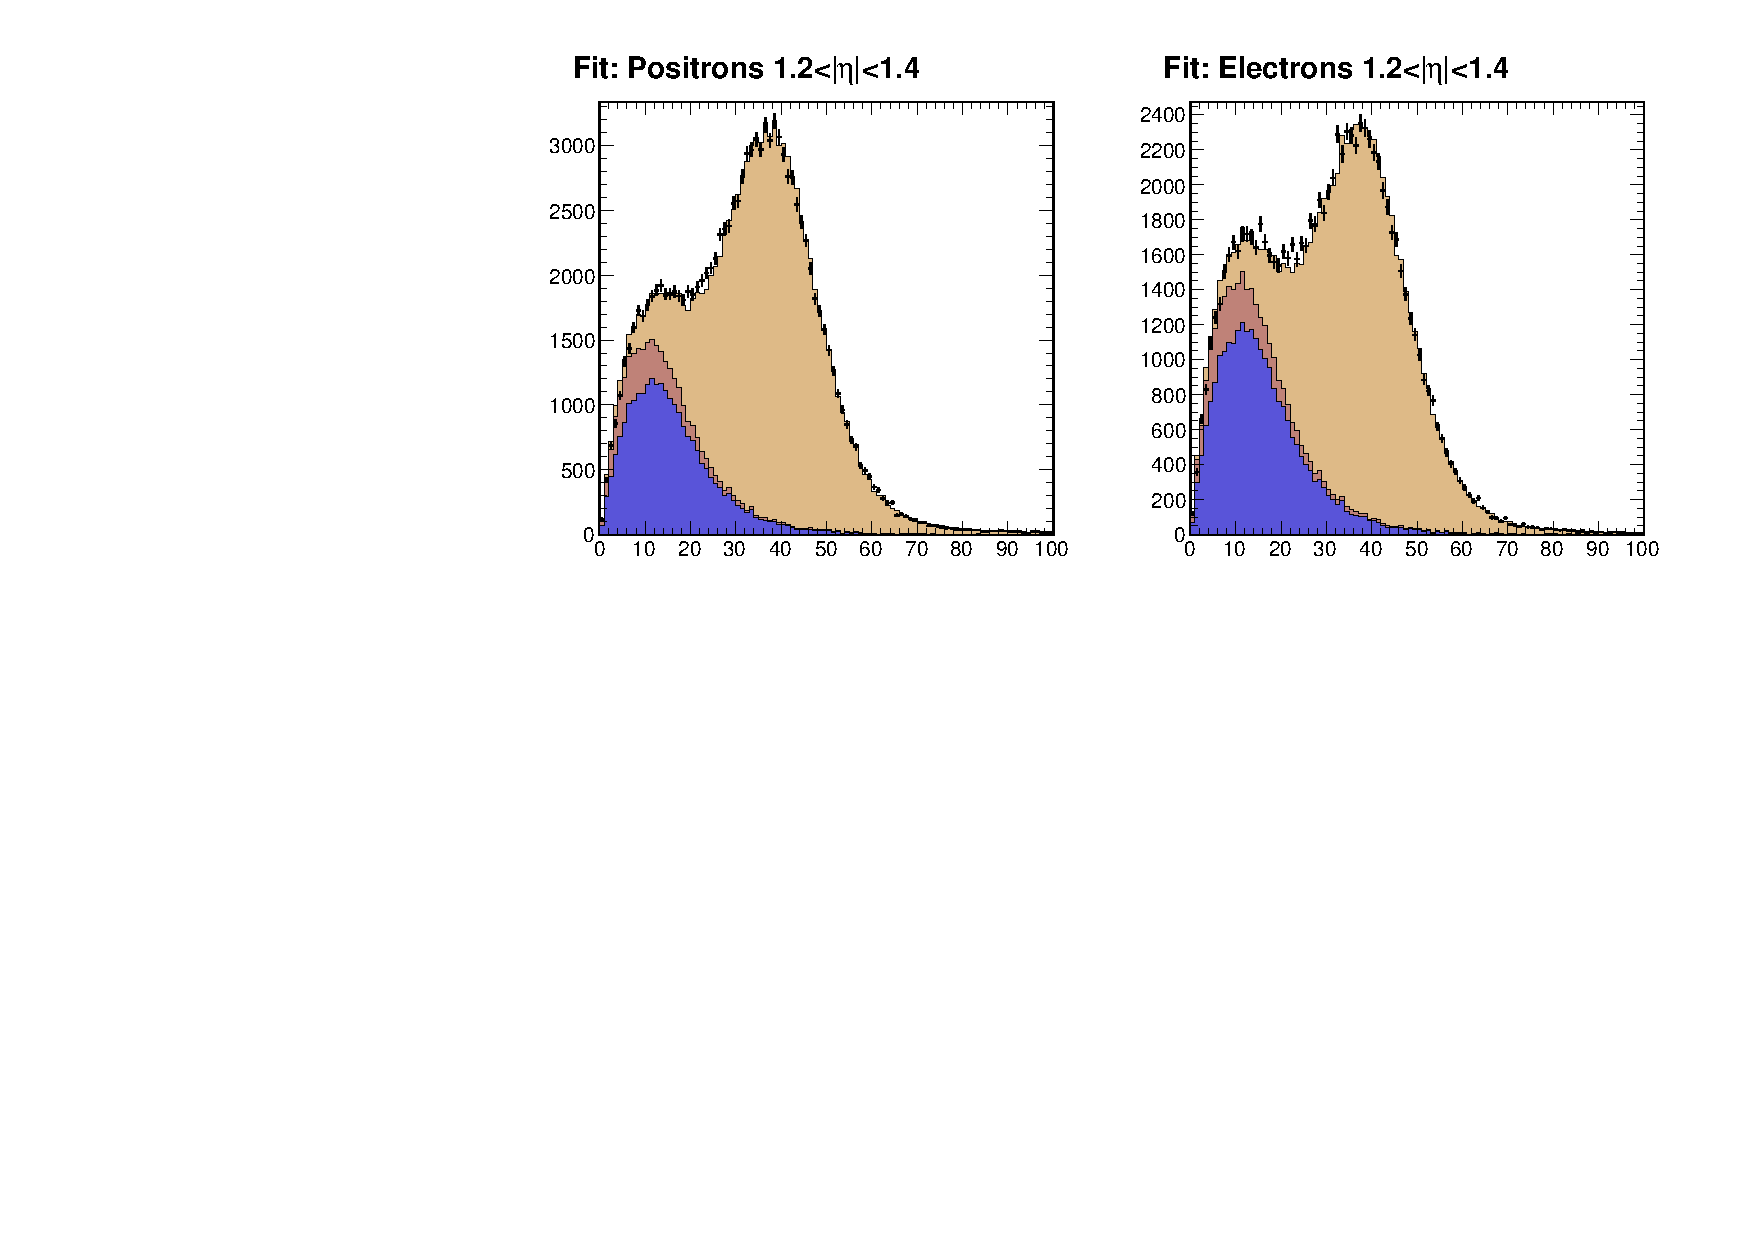
\includegraphics[width=0.95\textwidth]{data_6.pdf} \\
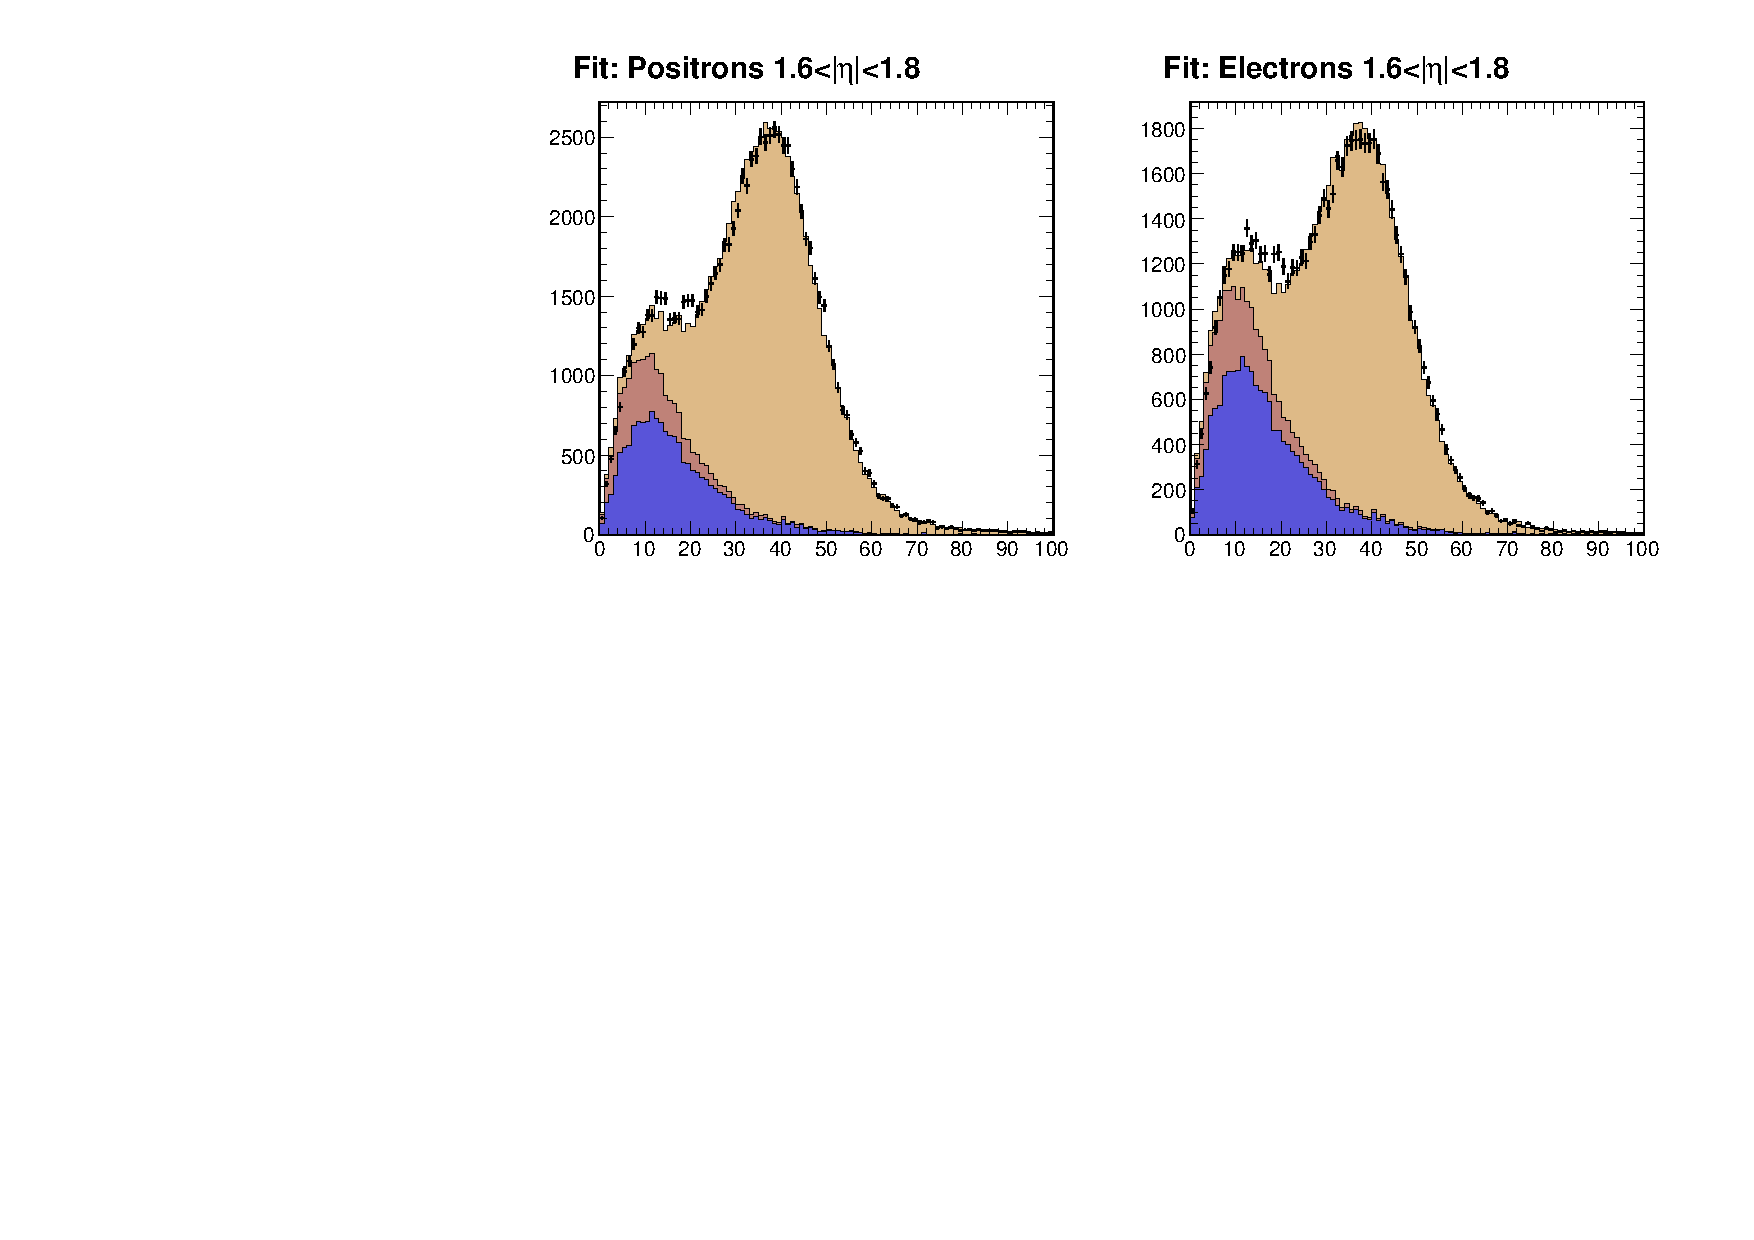
\includegraphics[width=0.95\textwidth]{data_7.pdf} \\
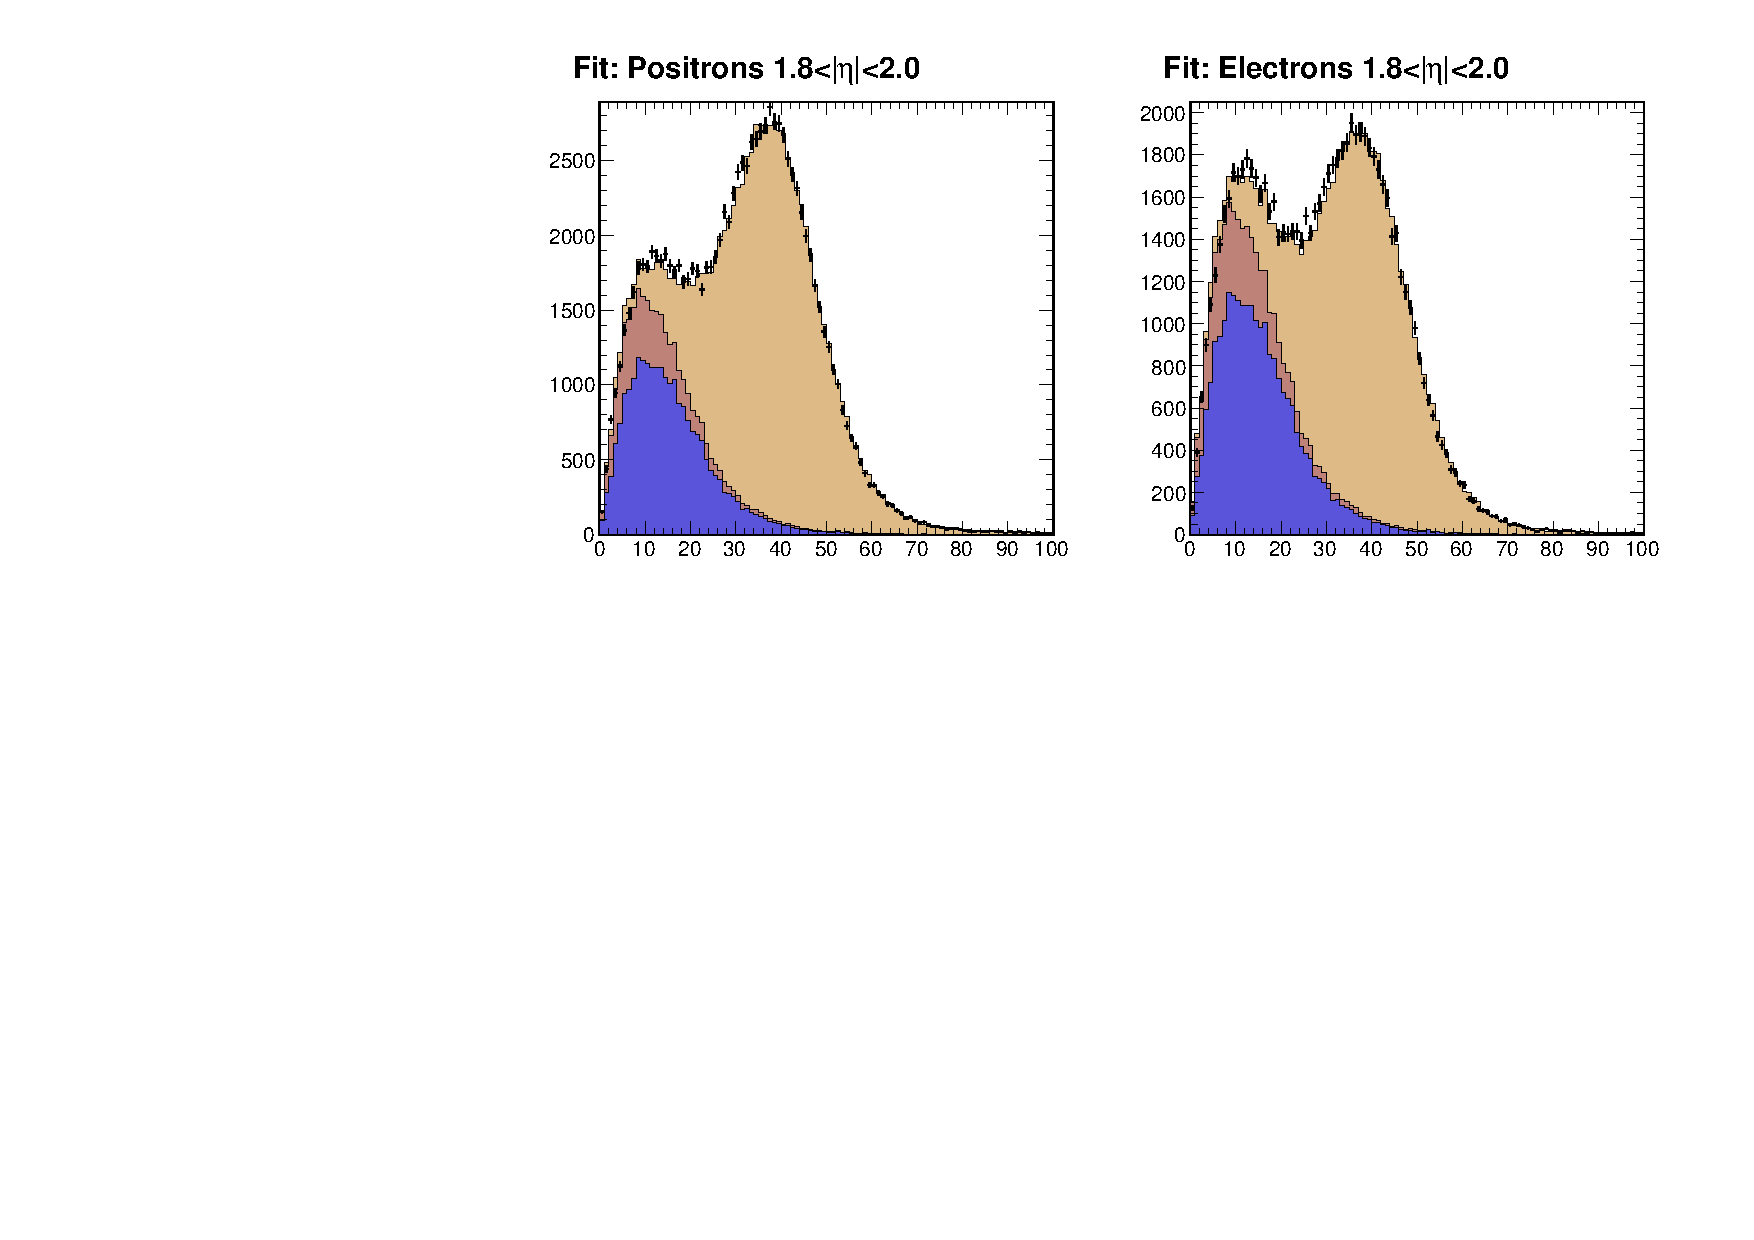
\includegraphics[width=0.95\textwidth]{data_8.pdf}
\caption[The fit to \MET for pseudorapidity bins 7,8 and 9.]
{\label{fig:data3} The fit to \MET\ for pseudorapidity bins 7,8 and
9.  The $x$-axis is the particle flow \ETm (GeV) and the $y$-axis is the number
of events ($\GeV^{-1}$).}
\end{center}
\end{figure}

\begin{figure}
\begin{center}
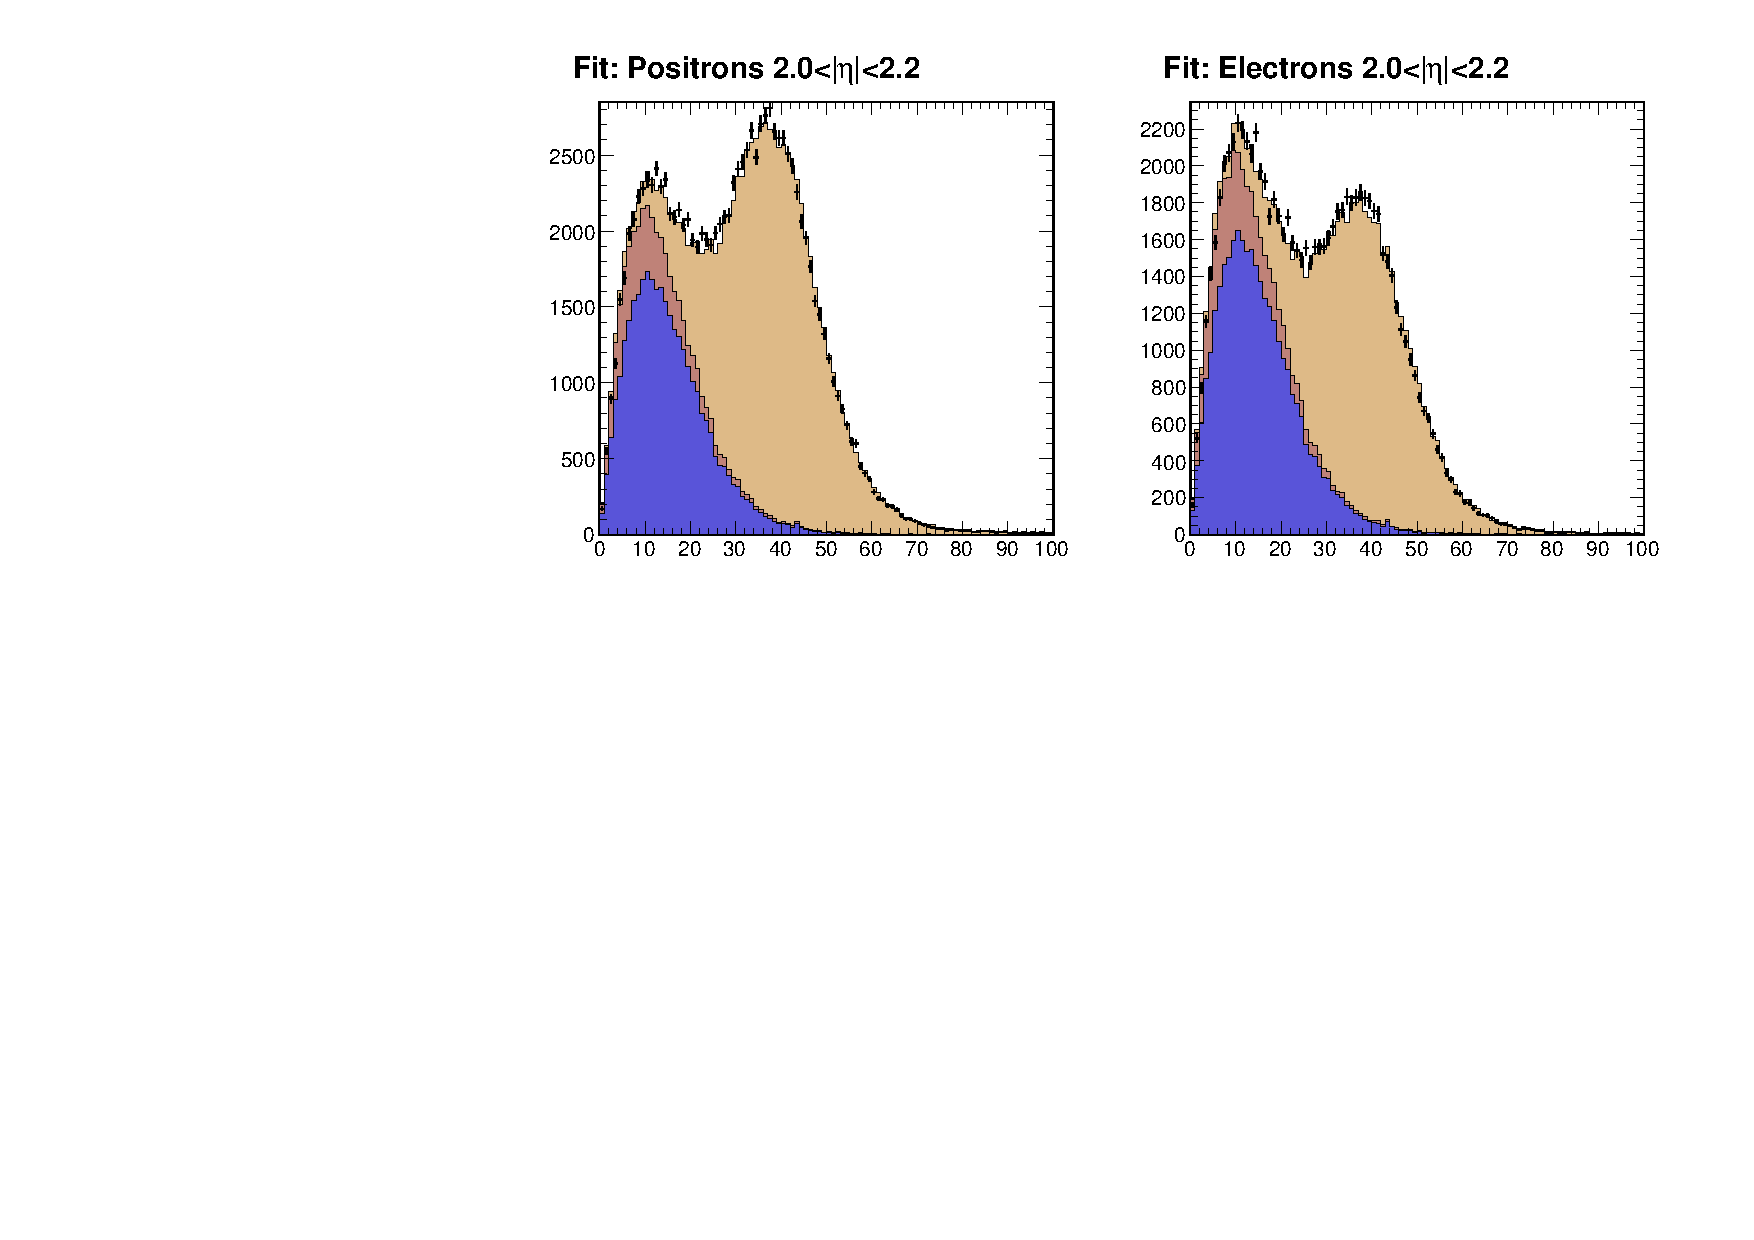
\includegraphics[width=0.95\textwidth]{data_9.pdf} \\
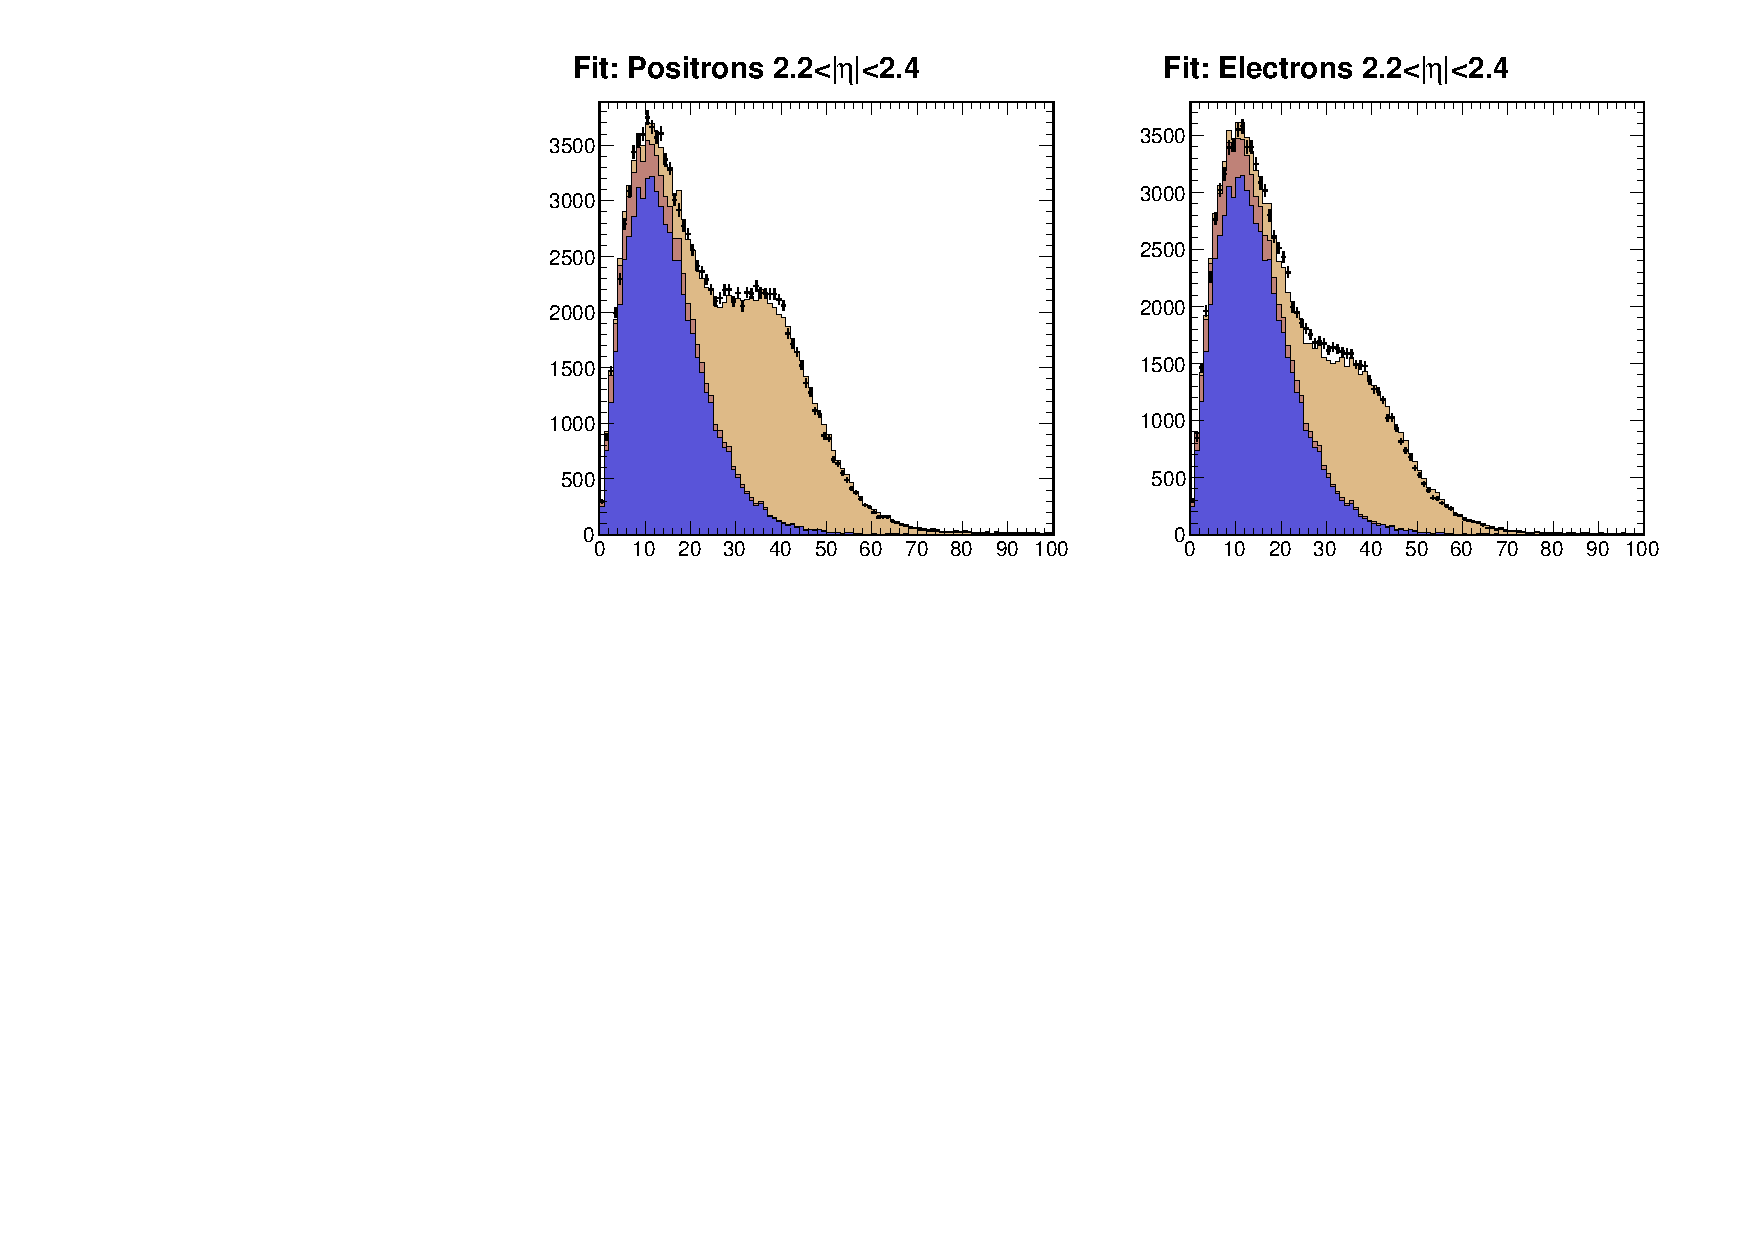
\includegraphics[width=0.95\textwidth]{data_10.pdf}
\caption[The fit to \MET for pseudorapidity bins 10,11 and 12.]
{\label{fig:data4} The fit to \MET\ for pseudorapidity bins 10 and
11.  The $x$-axis is the particle flow \ETm (GeV) and the $y$-axis is the number
of events ($\GeV^{-1}$).}
\end{center}
\end{figure}

